\chapter{Eletrônica}
\par A solução de eletrônica do projeto consiste em garantir todo o funcionamento eletrônico do projeto, que foi dividido em três subáreas: telemetria, sensoriamento e controle do abastecimento/ignição do foguete.
\par Como o principal objetivo do projeto é construir um sistema de controle e monitoramento do foguete que permita  ser feito a uma distância segura. Para isso, foi pensada uma solução envolvendo telemetria tanto para colher os dados quanto para enviar sinais de comando.Para melhor detalhamento da solução, foi construído um  \href{https://drive.google.com/file/d/12-pXv5L2Z5AuyWWVIr8VZ4WMghu7SYDw/view?usp=sharing}{Diagrama Geral}  para melhor detalhamento do projeto na parte de \textit{hardware}, a figura \ref{fig:Diagrama de Blocos} no apêndice \ref{Diagrama de blocos do sistema} resume bem a solução proposta.
 
\section{Telemetria}

\par É um processo remoto de aquisição ou envio de dados, ou seja, é utilizado para medir, rastrear ou até mesmo controlar à distancia alguma coisa. Esse processo é feito geralmente por um sistema de comunicação sem fio, como por exemplo por radiofrequência ou via satélite. \cite{Telemetria_AERONALTICA}.
\par Atualmente,  a telemetria está presente em diversos ramos da vida cotidiana do ser humano: na apuração das informações de um automóvel, no controle meteorológico, na agricultura e em outras diversas atividades.Para o projeto proposto, entende-se que o uso da telemetria em tempo real é extremamente vantajoso para a aquisição de dados durante o voo do foguete e para o controle autônomo do seu abastecimento/ignição.
\par Como requisito de segurança, é necessário fazer o controle  do foguete à distância. O recomendado pelas regras da LASC, competição a qual o cliente pretende participar, é uma distância mínima de 500m (lembrando que o foguete pode atingir uma altura de voo de aproximadamente 1km). Ou seja, fazer a aquisição de dados e o controle de abastecimento e ignição via cabo seria muito dispendioso, ou mesmo inviável, sujeito a maiores riscos de falhas, ou ficando na dependência de coletar os dados armazenados na memória do foguete somente após sua recuperação. Por essas razões, entende-se que é necessário realizar a telemetria em tempo real. Para melhor entendimento, na figura \ref{fig:Diagrama lançamento}   encontra-se o esquemático de um lançamento de foguete.

\begin{figure}[!htb]
\centering
\includegraphics[scale=0.5]{figuras/LANÇAMENTO.png}
\caption{Diagrama do Lançamento.}
{\footnotesize Fonte: Elaborado pelo autor.}
\label{fig:Diagrama lançamento}
\end{figure}

\par Como trata-se de uma função específica, o controle à distância e a aquisição de dados do pré-lançamento, do lançamento, do apogeu até a chegada do foguete no chão, é necessário compreender o problema e levantar requisitos para escolher a melhor forma de fazer a telemetria do projeto.
\par Foram analisadas diversas formas de fazer a telemetria, entre elas estão: a telemetria feita por radiofrequência, Lora, Wi-Fi, ZigBee, GPRS, Bluetooth, entre outras, analisando os seguintes requisitos: 
\begin{itemize}

\item Alcance;
\item Taxa de Transição de dados;
\item Protocolo de Comunicação;
\item Frequência dos Protocolos;
\item Potência de Transmissão; 
\item Interface de Dados;
\item Consumo.

\end{itemize}

\par Por fim, analisando diversos componentes, foi definido que a Placa Lora Esp32 da HELTEC, figura \ref{fig:Placa Esp32 Lora }, atende os requisitos do projeto citados acima, garantindo assim o funcionamento de qualidade do projeto, sendo que o principal motivo foi a distância alcançada pelo transmissor e a baixa perda de potência em sua transmissão.

\begin{figure}[!htb]
\centering
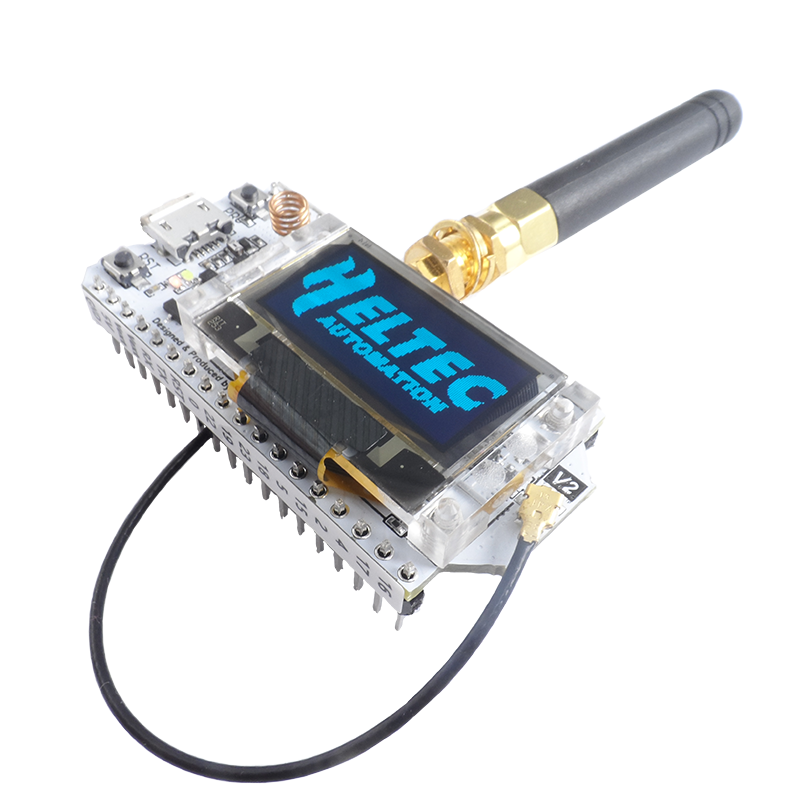
\includegraphics[scale=0.35]{figuras/SAM_0748_800X800.png}  
\caption{Placa Lora Esp32 da HELTEC.}
{\footnotesize Fonte:\cite{datasheet_ESP32}}
\label{fig:Placa Esp32 Lora }
\end{figure}
\par Contudo, como forma de garantir a integridade dos dados do lançamento, os mesmos também serão gravados num MicroSD dentro do foguete, evitando assim, a perda de dados por uma eventual falha na telemetria. 

\subsection{Lora}

\par A comunicação feita via Lora (Long Range) é um método de comunicação à distância sem fio, utilizando radiofrequência, pode ser considerado um marco para o IOT - internet das coisas, possibilitando a realização de diversos projetos com sua utilização.
\par A técnica de modulação utilizado pela LoRa é baseada na modulação \textit{Chirp Spread Spectrum} (CSS), que é bastante semelhante à modulação FSK (\textit{Frequency-shift keying}), onde a frequência varia linearmente ao longo do tempo. Contudo, o LoRa tem um ganho de potência maior em relação a modulação FSK, possibilitando assim maior alcance dos sinais.
\par A tecnologia LoRa possui uma uma estrutura de pacote de dados que pode variar entre 2 até 255 bytes, dependendo das configurações a serem utilizadas, além de ser possível alcançar uma taxa de transmissão de até 50 Kbps. Para isso, é necessário  utilizar artifícios e técnicas de canais \cite{transmissaoLoRa}. A LoRa pode ser utilizada em diversas bandas ISM (Industrial Sientific and Medical), que regula as frequências para livre desenvolvimento industrial, sendo que cada país tem seu órgão responsável para distinguir qual faixa pode ser utilizada, no Brasil se trata da ANATEL - Agência Nacional de Telecomunicações. Segundo a Resolução n$^{\circ}$ 726, de 05 de maio de 2020, que regulamenta as faixas livres de frequência no Brasil\cite{resolucao726}, a LoRa enquadra-se na faixa de frequência livre no Brasil, que varia de 902 a 928 MHz, entre outras, portanto o transmissor LoRa opera em 915MHz no continente americano se enquadrando na resolução supracitada, figura \ref{fig:Faixa de Frequência ISM}.

\begin{figure}[!htb]
\centering
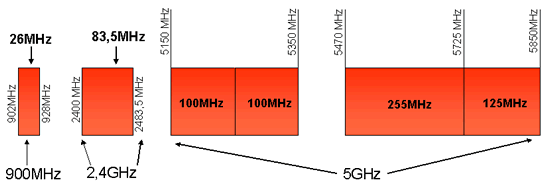
\includegraphics[width=\textwidth]{figuras/faixas de frequencia .png}  
\caption{Faixa de Frequência ISM no Brasil.}
{\footnotesize Fonte:\cite{faixafreq}}
\label{fig:Faixa de Frequência ISM} %\url{https://www.teleco.com.br/} }
\end{figure}
\par A modulação LoRa codifica a mensagem em pulsos de \textit{chirps}, sendo que possui alguns parâmetros importantes para o melhor entendimento do funcionamento do mesmo: a largura de banda, a frequência da portadora e a taxa de código\cite{desepenhoLoRa}.

\par A frequência da portadora é definida como a frequência central da informação, que é especificada pela região utilizada pelo equipamento (como citado anteriormente, a frequência é de 915MHz para o continente americano).

\par A largura de banda (\textit{Bandwidth} - BW) define o tamanho da faixa de frequência que a mensagem vai ser transmitida, ou seja a quantidade de informação que irá caber na mensagem. No protocolo de comunicação LoRa, há 3 configurações possíveis programáveis:  125KHz, 250KHz e 500KHz. Já o fator de espalhamento (\textit{Spreading Factor} - SF) determina a variação da duração do pulso \textit{chirps}, figura \ref{fig:sflora},sendo um parâmetro da modulação LoRa que tem como objetivo reduzir perdas na transmissão, porem há uma perda na taxa de transmissão. O SF pode variar de 7 até 12, ou seja, quanto maior o SF, maior será o tempo da mensagem no ar e, consequentemente, menor o tamanho da mensagem enviada. Na figura \ref{fig:sfloraDISTANCIA}, pode-se notar a representação dessa variante.

\begin{figure}[H]
  \centering
  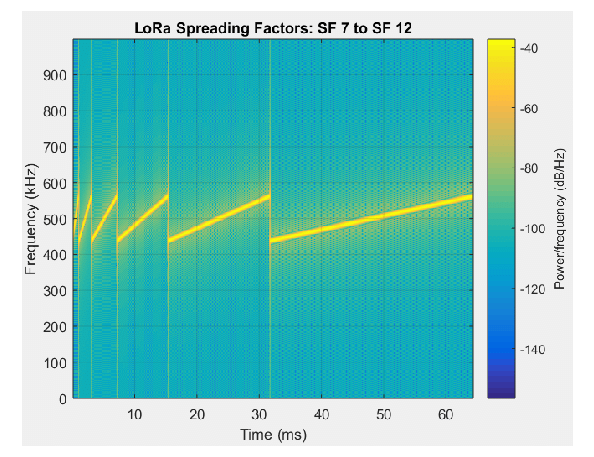
\includegraphics[scale=0.75]{figuras/sflora.png}
  \caption{Diferentes símbolos para SF diferentes em LoRa. }
 { \footnotesize Fonte:\cite{lorasf1}} 
  \label{fig:sflora}
\end{figure}

\begin{figure}[H]
  \centering
  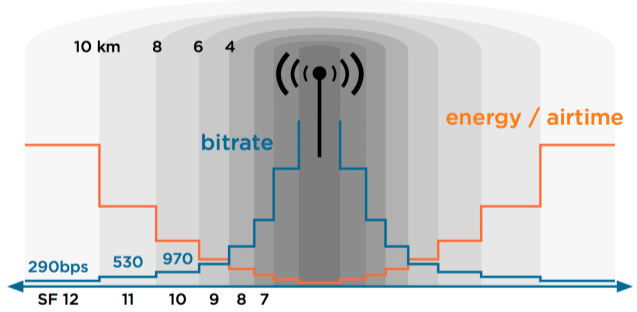
\includegraphics[width=\textwidth]{figuras/SFdistanci.png}
  \caption{Diferentes distancias para SF diferentes em LoRa. }
 { \footnotesize Fonte:\cite{lorasf}} 
  \label{fig:sfloraDISTANCIA}
\end{figure}

\par A taxa de código (\textit{Code Rate} - CR), é o modelo utilizado pela modulação LoRa para correção de erros na transmissão, é baseado em uma técnica correção posterior de erro, (\textit{Forward Error Corrector} - FEC). Portanto, o CR define a quantidade de bits de redundância serão utilizados na correção dos erros,  recuperando a mensagem, por sua vez, é dado pela equação \ref{cr} \cite{aplicacaolora}.

\begin{center}
\begin{equation}
\label{cr}
    CR=\frac{4}{4+n},\ com\  n \in \left\{1,2,3,4\right\}
\end{equation}
\end{center}

\par Por exemplo, usando n=1, temos um CR= $ \frac{4}{5}$, ou seja, $ \frac{1}{5}$ do pacote será composto por bits de redundância e os outros $ \frac{4}{5}$ serão compostos pela mensagem propriamente dita.

\par A taxa de bits (\textit{Bit Rate} - Rb) é a quantidade de bits que podem ser transmitidos por segundo em um determinado meio. Na modulação LoRa pode ser calculada pela equação \ref{taxa de bits }. Na figura \ref{fig:taxalora}, pode-se observar a variação da taxa de transmissão LoRa variando os parâmetros SF e a BW. 


%decidimos usar um SF entre 7 e 8, que atende nossa distancia pretendida com uma largura de banda de 500KHz e uma taxa de código de $ \frac{4}{5}$ ou$ \frac{4}{6}$que garante uma quantidade grande de dados a serem transmitidos.  

\begin{center}
\begin{equation}
 \label{taxa de bits }
 Rb =SF  \times \frac{BW \times CR } {2^{SF}}  ,\ com\  SF \in \left\{7,8,9,10,11,12\right\}
 \end{equation}

 \end{center}
Onde:

\begin{itemize}

\item Rb =Taxa de bits/s,
\item BW=Largura de banda(Hz),
\item SF=Fator de espalhamento,
\item CR=Taxa de código.

\end{itemize}

\begin{figure}[H]
  \centering
  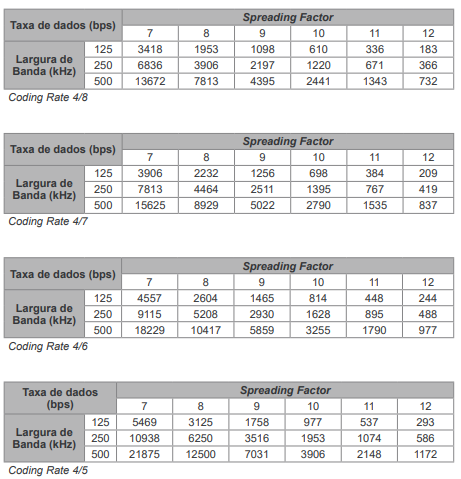
\includegraphics[width=\textwidth]{figuras/tabela de taxa lora.png}
  \caption{Diferentes taxa para SF e BW diferentes em LoRa. }
 { \footnotesize Fonte:\cite{aplicacaoloratabela}} 
  \label{fig:taxalora}
\end{figure}

\par Para configurações dos módulos SX1276 LoRa nas ESP 32 que compreende o trabalho em questão, foi feito levantamento dos dados a serem transmitidos e seu formato. A "Semtech" padronizou um formato especifico da mensagem para facilitar a conexões entres os transmissores e receptores sendo composta por (identificação + \textit{playload}), ou seja a identificação é o preâmbulo que é responsável pela si cronização entres o transmissor e receptor e o cabeçalho que é opcional que leva a informação do tamanho da mensagem e o \textit{playload} que é propriamente dito a mensagem mais os bits de redundância\cite{loras}.      
\par Ficou definido uma ordem fixa de agrupamento dos dados, assim, montando um pacote, além do mais que os dados seriam salvos  no formato em que os valores fossem separados por vírgulas (\textit{Comma Separated Values} - .CSV) que permite sua utilização de maneira mais prática tanto para seu armazenamento em banco de dados quanto para a criação de gráficos pertinente aos dados enviados.
\par Obtendo o tamanho de cada pacote, foi  analisado qual seria o pior caso para a transmissão, que no caso  é o pacote  de transmissão dos sensores de dentro do foguete para a RGS, este possui a string:\\
{ \footnotesize “InMSG, LATITUDE,LONGITUDE,TEMPERATURA,PRESSÃO,ALTITUDE,VELOCIDADE,Fimmsg”.}
\par A maior \textit{string} é constituída de 50 caracteres mais 6 vírgulas para separação dos dados, totalizando 56 caracteres, e sendo o maior pacote de dados que necessitará ser enviado. Dado que cada caractere possui 8 bits de acordo com o padrão da norma ISO/IEC 8859-16:2001, pode-se calcular o número de bits da maior \textit{string} a ser transmitida que contém aproximadamente 450 bits.

\par O cálculo das  para da taxa de transmissão é representado pela equação \ref{taxa de bits }, entretanto  \textit{Semtech} disponibiliza uma calculadora para levantamento dos dados da transmissão e recepção como apresentado nas figuras \ref{fig:calculo LoRa1}, \ref{fig:calculo LoRa2} em que foi definido os seguintes parâmetros dados as especificações do projeto, SF=8, BW=125 KHz, CR=$ \frac{4}{5}$,ou seja, um \textit{playload} de 68 bytes é necessário por estar-se usando o CR supracitado que acresce em $\frac{1}{5}$ o numero total de bits, sendo estes de redundância. Assim dado a frequência da portadora de 915 MHz e potência de transmissão de 20 dBm   obten-se uma taxa de transmissão de aproximadamente de 2000 bps suprindo com uma margem considerável  a demanda do projeto. 


\begin{figure}[H]
  \centering
  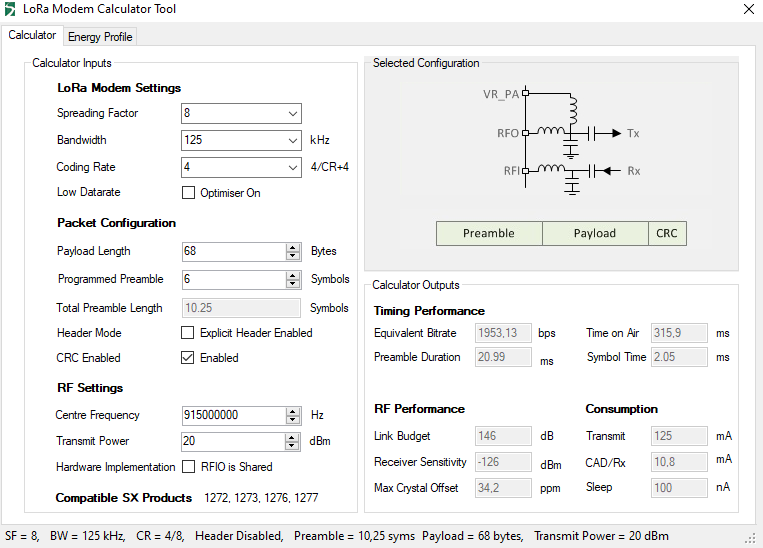
\includegraphics[scale=0.65]{figuras/calculo LoRa1.1.png}
  \caption{Cálculo transmissão LoRa pela Sentech. }
 { \footnotesize Fonte: Semtech - LoRa Modem calculator Tool} 
  \label{fig:calculo LoRa1}
\end{figure}


\begin{figure}[H]
  \centering
  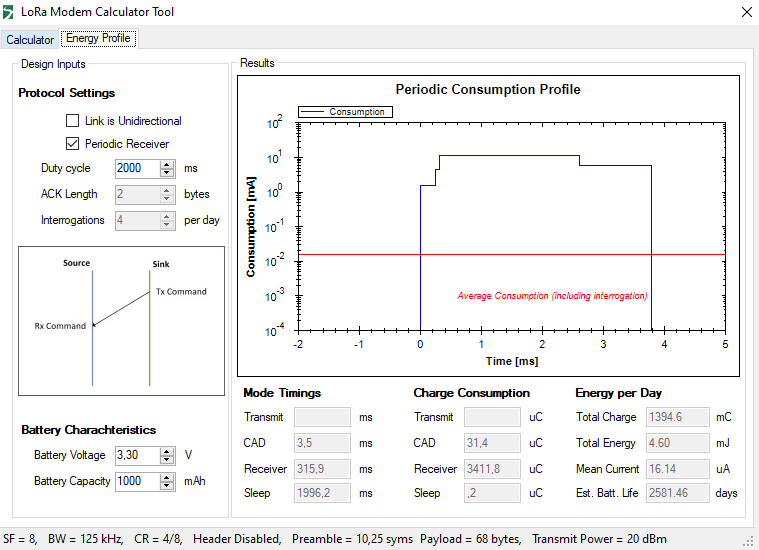
\includegraphics[scale=0.65]{figuras/calculo LoRa1.2.png}
  \caption{Cálculo transmissão LoRa pela Sentech. }
 { \footnotesize Fonte:Semtech - LoRa Modem calculator Tool} 
  \label{fig:calculo LoRa2}
\end{figure}


\section{Sensoriamento}

\par Sensores são dispositivos que possuem a função de detectar e responder com eficiência algum estímulo. Existem vários tipos de sensores que respondem a estímulos diferentes, como por exemplo: calor, pressão, movimento, luz e outros. Depois que o sensor recebe o estímulo, a sua função é emitir um sinal que seja capaz de ser convertido e interpretado pelos outros dispositivos \cite{mattede_Sensores_blog2020}.

\par Definidos os requisitos do projeto, sabe-se que será necessário o uso de sensores e transdutores para auxiliar a obter dados como pressão, temperatura, altitude, velocidade e localização geográfica (GPS) do foguete, e também do peso do foguete durante o abastecimento na sua base de lançamento. Para tal, serão utilizados apenas 3 sensores para ajudar na busca dessas variáveis.

\subsection{Altitude e Velocidade}

\par Para medição da pressão e da temperatura externa ao foguete durante o lançamento, foi escolhido o sensor de pressão e temperatura BMP280, visto na figura \ref{fig:sensor_pressao} \cite{datasheet_BMP280}.

\begin{figure}[H]
  \centering
  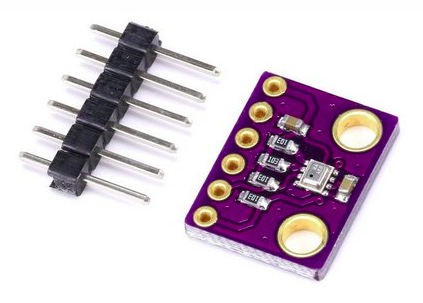
\includegraphics[scale=0.75]{figuras/BMP280.png}
  \caption{Sensor de pressão e temperatura BMP280 (Bosch). }
 { \footnotesize Fonte:\cite{figura_BMP280}} 
  \label{fig:sensor_pressao}
\end{figure}

\par Esse sensor mostrou-se o mais viável, pois, implementando-o com uso de determinadas bibliotecas, além dos dados de pressão (hPa) e temperatura (Graus Celsius), é possível, por meio da implementação de funções contidas em bibliotecas especificas, obter o cálculo da altitude (metros). Tais bibliotecas e suas equações são esclarecidas adiante.

\par O sensor BMP280 realiza medições de pressão com precisão de $\pm$ 1 hPa e temperatura com precisão de $\pm 1 ^\circ C $. Com essa precisão, é possível realizar medições de altitude com margem de erro de  $\pm$ 1 metro, efetuando a leitura entre 300 e 1100 hPa, o que corresponde à faixa de altitude de +9000 à -500 m \cite{cia_BMP280_2017}.

\par Em relação aos sensores existentes no mercado, o BMP280 foi o que melhor atendeu aos requisitos, pois ele é a versão mais atual e precisa dos modelos BMP180 e BM085. Também é de baixo consumo em relação aos sensores Mpx10dp e Mpx5700, possuindo melhor aplicabilidade.

\par Para a implementação do sensor, é necessário o uso de duas bibliotecas da Adafruit para o sensor BMP280 \cite{Adafruit}: a  \href{https://github.com/adafruit/Adafruit_BMP280_Library}{Adafruit\textunderscore Sensor.h} e a \href{https://github.com/adafruit/Adafruit_Sensor}{Adafruit\textunderscore BMP280.h}. Em ambientes que a Adafruit não pode ser implementada, a Bosh, fabricante do sensor, disponibiliza um código em C para a sua implementação (em \href{https://github.com/BoschSensortec/BME280_driver}{BME280\textunderscore driver}).

\par A biblioteca \href{https://github.com/adafruit/Adafruit_Sensor}{Adafruit\textunderscore BMP280.h} citada anteriormente é a biblioteca que disponibiliza as funções, em código C, que retornam as medidas de pressão e temperatura, e também a função que já realiza o cálculo da altitude, tais funções são:

	\begin{itemize}
	    \item float readPressure() -> Leitura da Pressao atmosférica
	    \item float readTemperature() -> Leitura da Temperatura
	    \item float readAltitude -> Leitura da Altitude (em metros, considerando nível do mar)
	\end{itemize} 

\par Os dados retornados por cada uma dessas funções são do tipo \textit{float}, portanto cada medida tem o dado do tamanho de 4 bytes.

\par A função \textit{readAltitude()} retorna o valor da altitude por meio da equação hipsométrica, vide equação \ref{eq_hipsometrica}. A equação hipsométrica estabelece que a distância vertical entre duas pressões na atmosfera é proporcional à temperatura média entre esses dois níveis de pressão \cite{hipsometric}.

\begin{center}
\begin{equation}
\label{eq_hipsometrica}
h=z_{2}-z_{1}=\frac{R_{d} \overline{T_{\nu}}}{g} \ln \left(\frac{p_{1}}{p_{2}}\right)
\end{equation}
\end{center}

Onde:
\begin{itemize}
    \item h é a variação da altitude, em que $z_{1}$ e $z_{2}$ são alturas geométricas nos níveis de pressão $p_{1}$ e $p_{2}$;
	\item $R_{d}$ é a constante de gás para ar seco, $8,3144 \frac{N*m}{mol*K}$ ;
	\item $\overline{T_{\nu}}$ a temperatura virtual média da camada;
	\item g é a aceleração gravitacional, $9.807 \frac{m}{s^{2}}$ .
\end{itemize} 

\par A equação hipsométrica é derivada da equação hidrostática e da lei dos gases ideais. Com essa fórmula a função calcula a altura h com, $p_{1}$ sendo a pressão atmosférica medida pelo sensor BMP280 e $p_{2}$ a pressão inicial da altura inicial, podendo ser a pressão a nível do mar (101,35 kPa) ou a do local.

\par Sabendo a altitude do foguete e obtendo a sua variação ao longo do tempo, este podendo ser medido pelo  \textit{clock} próprio do microcontrolador, considerando o tempo de recebimento de cada medida de altitude, é possível medir a velocidade do foguete em cada instante, por meio do cálculo da velocidade média, equação \ref{eq_vel_media}.

\begin{center}
\begin{equation}
\label{eq_vel_media}
V = \frac{\Delta S} {\Delta T} = \frac{h_{f} - h_{i}}{t_{f} - t_{i}}
\end{equation}
\end{center}

\par Onde:

\begin{itemize}
    \item V é a velocidade média do foguete durante o voo, em m/s;
	\item $\Delta$S é a variação de altitude do foguete durante o voo, em metros;
	\item $\Delta$T é a variação de tempo de subida do foguete durante o voo, em segundos;
	\item $h_{f}$ é a última medida coletada da altura do foguete;
	\item $h_{i}$ é a penúltima medida coletada da altura do foguete, esta inicia na altura h = 0 metros;
	\item $t_{f}$ é a medida do tempo em que foi coletado $h_{f}$;
	\item $t_{i}$ é a medida do tempo em que foi coletado $h_{i}$, está inicia em 0 segundos.
\end{itemize}

\par Ao contrário do cálculo da altitude, que é obtida por hardware dentro de rotinas implementadas em código C no microcontrolador, o processamento e cálculo da velocidade média do foguete, será realizado por software. A função do microcontrolador, nesse caso, será de enviar os dados de altitude para tal procedimento. 

\par Usando a comunicação I2C, a conexão das pinagens entre o sensor e o microcontrolador foi definida com o SDA e SCL do BMP280 conectados aos pinos D21 e D22 da ESP32 LoRa,respectivamente. Para comunicação, foram conetados o VDD e GND do BMP280 com os pinos 3V3 e GND da ESP32 LoRa respectivamente, conforme mostrado na figura \ref{fig:PINAGEM_BMP280}. 

\begin{figure}[H]
  \centering
  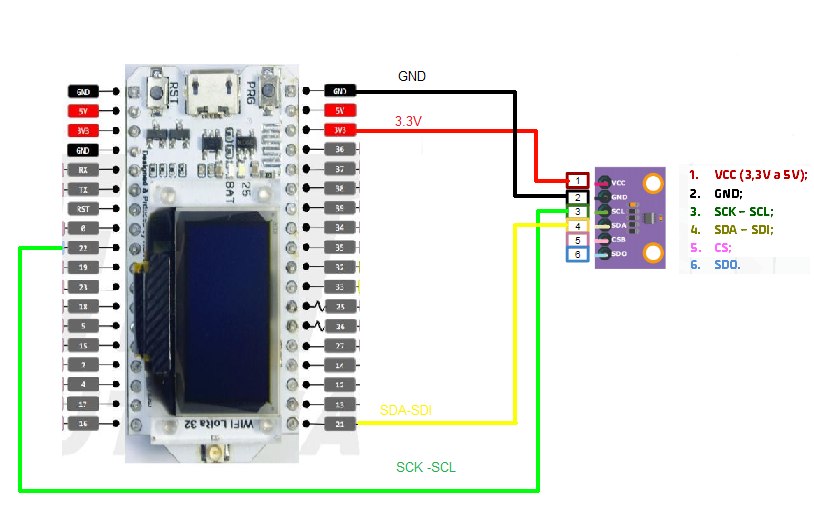
\includegraphics[scale=0.35]{figuras/PINAGEM_BMP280.png}
  \caption{Conexões entre sensor BMP280 e ESP32 LoRa - Protocolo I2C.} 
  {\footnotesize Fonte : Autor } 
  \label{fig:PINAGEM_BMP280}
\end{figure}

\subsection{Localização Geográfica (GPS)}

\par A sigla GPS significa Global Positioning System, o que em português quer dizer Sistema de Posicionamento Global. É uma tecnologia que utiliza satélites e dispositivos para fornecer informações sobre a localização no globo terrestre \cite{fisica_GPS_2020}.
\par A localização GPS será utilizada para obter a posição geográfica do foguete após sua aterrissagem, podendo também fornecer as coordenadas ao longo do lançamento para determinar a trajetória percorrida pelo foguete.
\par Foi definido para tal função o GY-NEO6MV2, figura \ref{fig:moduloGPS}, um módulo GPS composto por duas partes, a antena, responsável por captar as informações provindas dos satélites e o sistema de controle, responsável pelo processamento dos dados obtidos, por meio do microcontrolador interno NEO6 \cite{datasheet_GPS}.

\begin{figure}[H]
  \centering
  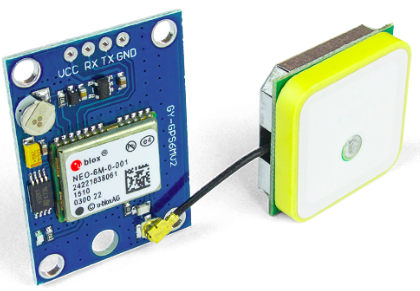
\includegraphics[scale=0.6]{figuras/moduloGPS.png}
  \caption{Módulo GPS GY-NEO6MV2 (uBlox). }
  {\footnotesize Fonte: \cite{figura_GPS}}
  \label{fig:moduloGPS}
\end{figure}

\par O módulo GPS GY-NEO6MV2 foi escolhido por ser de fácil utilização, realizando a comunicação por meio de comunicação serial, usando apenas 2 pinos (TX e RX), o que permite a comunicação com os mais diversos tipos de equipamentos e microcontroladores. Esse componente apresenta um consumo de corrente em média de 45 mA, enquanto o módulo similar, VK2828U7G5LF, consome em média 50 mA.

\par Para a aplicação com o módulo é necessário o uso de duas bibliotecas essenciais. A primeira é para a realizar a comunicação serial do microcontrolador com o módulo GPS, onde pode ser usada tanto a biblioteca \href{https://www.arduino.cc/en/Reference/softwareSerial}{SoftwareSerial.h} para usar a IDE do arduino, quanto a biblioteca \href{https://github.com/plerup/espsoftwareserial}{EspSoftwareSerial.h} como exclusivo da ESP32. A segunda (\href{https://github.com/mikalhart/TinyGPS}{TinyGPS.h}) contém todas as funções e comandos necessários para se comunicar com o módulo e acessar suas ferramentas.

\par Para GPS GY-NEO6MV2, com a vantagem da sua comunicação ser serial, a sua pinagem com a WiFi Lora ESP32 é bastante simples. Portanto, foi definida a conexão dos pinos de VCC e GND do módulo com os pinos 3V3 e GND da ESP32, para alimentação, e conectamos o TX e RX do módulo com os pinos de RX e TX da ESP32 LoRa, usando o procotolo UART de comunicação. A figura \ref{fig:PINAGEM_GPS} mostra as conexões entre os componentes.

\begin{figure}[H]
  \centering
  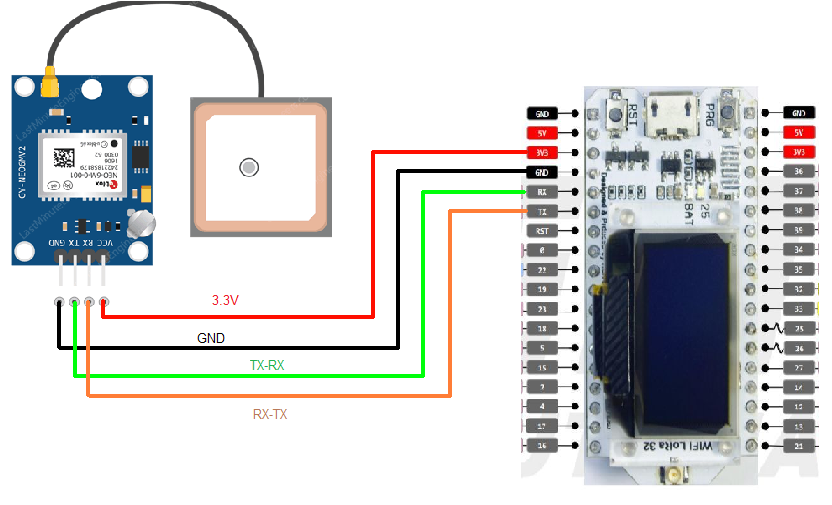
\includegraphics[scale=0.4]{figuras/PINAGEM_GPS.png}
  \caption{Conexões entre o GPS GY-NEO6MV2 e ESP32 LoRa - Protocolo UART.} 
  {\footnotesize Fonte : Autor } 
  \label{fig:PINAGEM_GPS}
\end{figure}


\subsection{Peso do foguete}
\label{Peso_do_Foguete}

\par Por meio do acompanhamento do peso do antes, durante e depois do abastecimento do foguete, será possível controlar e medir a quantidade de combustível contido em seu tanque. Para mensurar o peso do foguete, serão utilizadas duas células de carga. 

\par Uma célula de carga é um transdutor de força que converte a carga que atua sobre ele em uma saída elétrica mensurável. Embora existam vários tipos, as células de carga baseadas em sensores de deformação e tensão são as mais usadas \cite{omega_celulacarga}. 

\par Neste projeto, foi escolhida célula de carga de 50 kg, figura \ref{fig:celula_carga}, que atende o peso máximo do foguete, de 18.5 kg com o tanque de combustível cheio e 14.3 kg vazio (dados fornecidos pela CRT).

\begin{figure}[H]
  \centering
  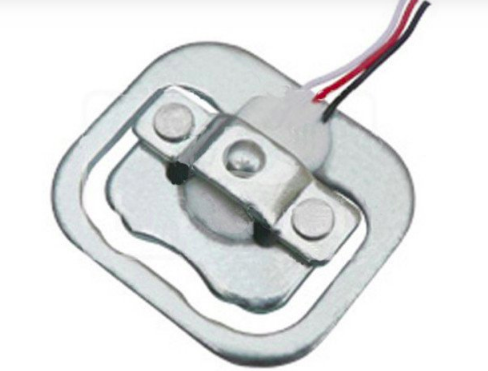
\includegraphics[scale=0.5]{figuras/celula_carga.png}
  \caption{Célula de carga - 50 kg.}
  {\footnotesize Fonte: \cite{figura_celula}} 
  \label{fig:celula_carga}
\end{figure}

\par Este sensor é um \textit{Strain Gauge}, ou extensômetro, um sensor que é colocado na superfície de uma peça, responsável por medir a deformação diante da aplicação de um carregamento, onde no sensor há um fio resistivo, que altera sua resistência de acordo com o “alongamento” da superfície em que está colocado, gerando assim sinais elétricos que são interpretados por uma placa de aquisição, convertendo os valores em deformação \cite{strain_gauge}.

\par Uma ponte Wheatstone é um esquema de montagem de elementos elétricos que permite a medição do valor de uma resistência elétrica desconhecida, vide Figura \ref{fig:ponte_wheatstone}. Neste esquema elétrico são ligados quatro resistores, em dois diferentes ramos de um circuito, a uma bateria. Em seguida, esses ramos são conectados por um fio, que os leva a um galvanômetro. O galvanômetro serve como um indicador de corrente elétrica, assim, a resistência do resistor variável é alterada  até que o galvanômetro acuse a passagem de corrente nula. Quando a corrente que passa pelo galvanômetro é nula, não há diferença de potencial entre os ramos do circuito. Nessa situação, dizemos que a ponte de Wheatstone encontra-se em equilíbrio.

\begin{figure}[H]
  \centering
  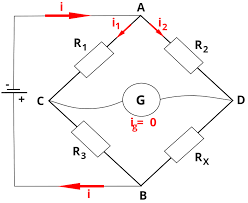
\includegraphics[scale=0.6]{figuras/ponte_wheatstone.png}
  \caption{Circuito padrão de uma Ponte de Wheatstone.}
  {\footnotesize Fonte: \cite{ponte_wheatstone}} 
  \label{fig:ponte_wheatstone}
\end{figure}

\par Onde $i_{g}$ é a corrente no galvanômetro, $R_{X}$ é a resistência desconhecida e $R_{1}$, $R_{3}$, $R_{3}$ são resistências conhecidas. Na situação de equilíbrio, $i_{g} = 0$, o circuito mostrado na figura anterior pode ser usado para determinar com grande precisão a resistência elétrica do elemento resistivo RX. 
\par A célula de carga utilizada, é um sensor de meia-ponte da \textit{Wheatstone}, ou seja, utiliza uma meia-ponte de \textit{Wheatstone} com uma resistência de referência e um elemento sensor cuja resistência varia conforme a pressão aplicada, vide Figura \ref{fig:half_wheatstone}. Utilizando-se apenas uma célula de carga seriam necessários mais resistores para completar a ponte. Além disso, projetos com apenas uma célula de carga tendem a ter dificuldades para ajustes de calibração da célula.

\begin{figure}[H]
  \centering
  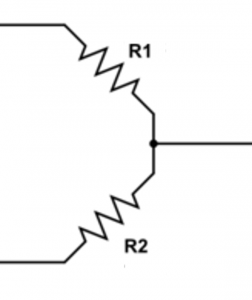
\includegraphics[scale=0.6]{figuras/half_wheatstone.png}
  \caption{Circuito Meia-Ponte de Wheatstone da Célula de Carga utilizada.}
  {\footnotesize Fonte: \cite{half_wheatstone}} 
  \label{fig:half_wheatstone}
\end{figure}

\par Portanto, considerando também que, além do foguete acima da balança, haverá toda uma estrutura para comportar a base do foguete, serão usadas duas células de cargas para fazer a balança, o que é o mais indicado: uma para medir compressão e outra para medir tensão (forças aplicadas em direções diferentes). Com duas células de carga, tem-se uma ponte de \textit{Wheatstone} completa.

\par Como o sinal enviado pelo transdutor é elétrico, precisa-se de um módulo conversor, que fará a conversão do sinal elétrico em sinal digital para possibilitar a leitura dos dados pelo microcontrolador. Para isso, será usado o módulo conversor A/D HX711, figura \ref{fig:conversorHX711}, um módulo amplificador e conversor A/D de 24 bits, utilizado para amplificar o sinal de dispositivos como células de carga, fazendo a interligação entre essas células e o microcontrolador, por meio da comunicação SPI \cite{avia_HX711}.

\begin{figure}[H]
  \centering
  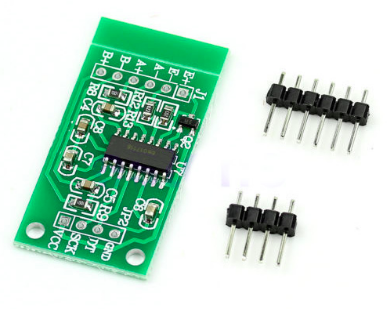
\includegraphics[scale=0.6]{figuras/conversorHX711.png}
  \caption{HX711 - Módulo amplificador e conversor A/D de 24 bits.}
  {\footnotesize Fonte: \cite{figura_HX711}} 
  \label{fig:conversorHX711}
\end{figure}

\par O módulo HX711 foi projetado para pesar escalas e aplicações de controle industrial para interface diretamente com um sensor de ponte. O multiplexador de entrada seleciona o Canal A ou entrada diferencial B para o baixo ruído amplificador de ganho programável (PGA). O Canal A pode ser programado com um ganho de 128 ou 64,
correspondendo a uma entrada diferencial em escala real tensão de ± 20mV ou ± 40mV, respectivamente, quando uma fonte de 5 V é conectada à alimentação analógica do AVDD, pino de alimentação. O canal B tem um ganho fixo de 32. O regulador de alimentação Onchip elimina a necessidade para um regulador de alimentação externa fornecer energia para o ADC e o sensor. A entrada do \textit{Clock} é
flexível, pode ser de uma fonte de relógio externa, um
cristal, ou um oscilador on-chip que não requer nennhum componente externo. Não há necessidade de programação para os
registradores internos, todos os controles do HX711 são
através dos pinos \cite{avia_HX711}.

\par A Figura \ref{fig:bloco_H711}, mostra o diagrama de bloco de aplicação de uma balança típica com o HX711, dentro do bloco em azul, e a célula de carga, uma ponte de Wheatstone externa ao bloco. Em destacado em azul está o diagrama de bloco interno do módulo HX711.

\begin{figure}[H]
  \centering
  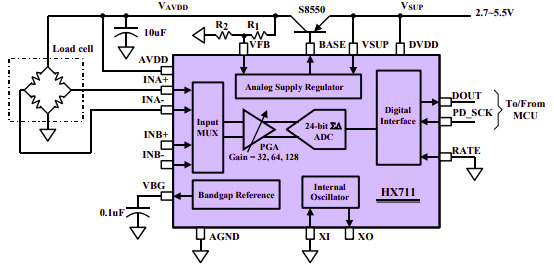
\includegraphics[scale=0.4]{figuras/blocoHX711.jpeg}
  \caption{Diagrama de blocos do módulo HX711 em aplicação típica de uma balança com uma célula de carga.} 
  {\footnotesize Fonte : \cite{avia_HX711} } 
  \label{fig:bloco_HX711}
\end{figure}

Aplicando ao presente projeto, a conexão das duas células de carga, formando a ponte completa de Wheatstone, e o módulo HX711, fica conforme mostrado na Figura \ref{fig:Circuit_balanca}.

\begin{figure}[H]
  \centering
  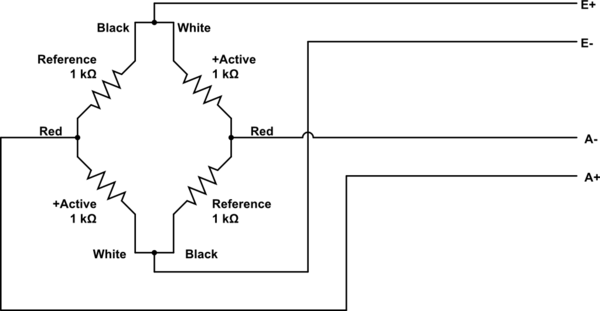
\includegraphics[scale=0.4]{figuras/Circuit_balanca.png}
  \caption{Circuito com 2 células de carga com conexões para o módulo HX711.} 
  {\footnotesize Fonte : \cite{half_wheatstone} } 
  \label{fig:Circuit_balanca}
\end{figure}

\par Para implementar a balança, a comunicação é feita do microcontrolador com o módulo conversor A/D e amplificador HX711. Para tal, foi definido o protocolo de comunicação I2C, sendo necessário o uso da biblioteca \href{https://github.com/bogde/HX711}{HX711.h}. Nessa biblioteca, a função a ser utilizada,  que retorna os dados do peso da balança é do tipo \textit{long}, ou seja, uma dado de 4 bytes.

\par As conexões entre o conversor e microcontrolador foram definidas da seguinte forma: para alimentação, o VDD e GND do HX711 conectados nos pinos 5V e GND da ESP32 Lora, respectivamente, para comunicação I2C, o DT e SCK do HX711 conectados nos pinos D23 e D17 da ESP32 LoRa. A figura \ref{fig:PINAGEM_balanca} mostra as pinagens realizadas.  

\begin{figure}[H]
  \centering
  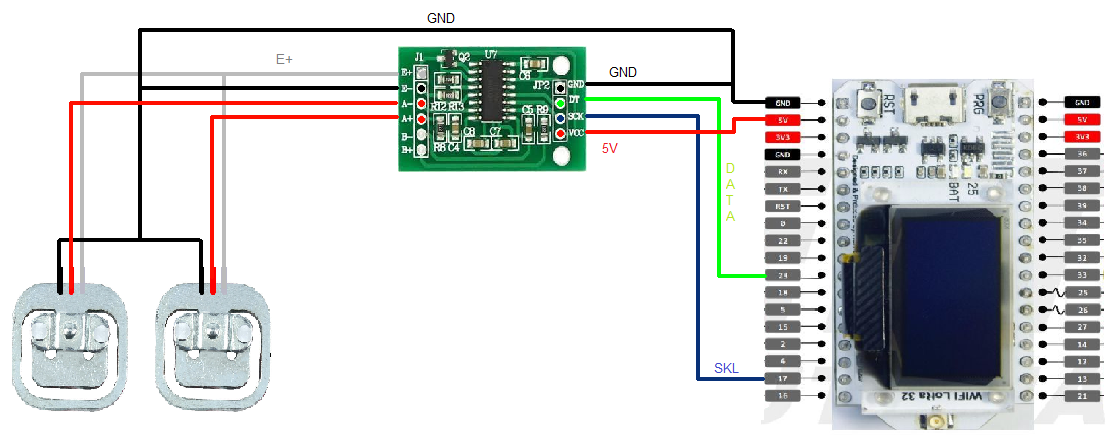
\includegraphics[scale=0.4]{figuras/PINAGEM_BALANCA.png}
  \caption{Conexões entre Hx711 e ESP32 LoRa - Protocolo I2C.} 
  {\footnotesize Fonte : Autor } 
  \label{fig:PINAGEM_balanca}
\end{figure}

\subsection{Especificações dos sensores}

\par A tabela \ref{tab:sensores} apresenta os dados das principais especificações dos sensores citados acima.

\begin{center}
\begin{table}[H]
\centering
\begin{tabular}{ |m{2cm}|m{2cm}|m{2.5cm}|m{2.5cm}|m{2.5cm}|m{2.5cm}| } 
\hline

\textbf{ Sensor }&\begin{center}
\textbf{ Tensão de Operação} \end{center}& \textbf{Consumo de corrente }& \textbf{Comunicação} & \begin{center}\textbf{Taxa de transmissão} \end{center} & \begin{center}\textbf{Formato dos Dados}\end{center}\\ 
 \hline
 
 BMP280 & 1.71 - 3.6V & 3.6 $\micro$uA @ 1 Hz (umidade, pressão e temperatura) & 
I2C e SPI & I2C (até 3.4 MHz e SPI (3 e 4 fios, até 10 MHz) & unsigned 20-bit (pressão e temperatura) unsigned 16-bit (umidade)\\
  \hline
Célula de carga 50kg & 5 -10V & Resistência de entrada e saída ($\ohm$): 1000 ± 50 & - & - & - \\
  \hline
 Módulo Hx711 & 4.8 - 5.5V & 1.5mA & SPI & 10 - 80 MHz & 24 bits em complemento de 2 \\ 
  \hline
 Módulo GPS GY-NEO6MV2 & 3 - 5V & 10mA – 100 mA & Serial UART e SPI & 9600 bps (UART baud rate) e 100 kbit/s & - \\ 
 \hline 

\end{tabular}
\caption{Especificações principais dos componentes do sensoriamento.}
\label{tab:sensores}
\end{table}
\end{center}


\section{Central de controle}

\par A central de controle será o ponto de acesso do usuário com os dados e comandos vindos da base de lançamento e do foguete. Um exemplo de estação pode ser visto na figura \ref{fig:DroneStation}. 

\begin{figure}[H]
  \centering
  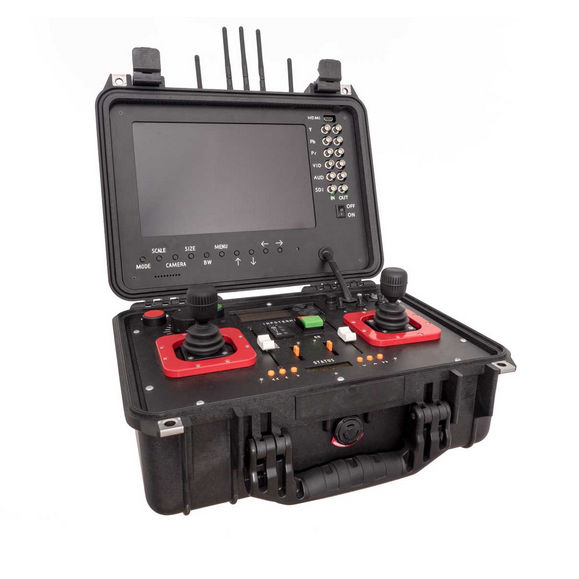
\includegraphics[scale=0.4]{figuras/DroneGroundStation.jpg}
  \caption{Estação de controle de solo.}
  {\footnotesize Fonte : \cite{AeroExpo}} 
  \label{fig:DroneStation}
\end{figure}


\par A solução proposta para essa interface do usuário foi seguindo esse modelo de maleta, que possui uma tela, um teclado.

\subsection{Interface do usuário}

\par A tela escolhida pode ser vista na figura \ref{fig:Tela}. Essa tela possui um tamanho de 9 polegadas e uma resolução máxima de 1600x1200. 


\begin{figure}[H]
  \centering
  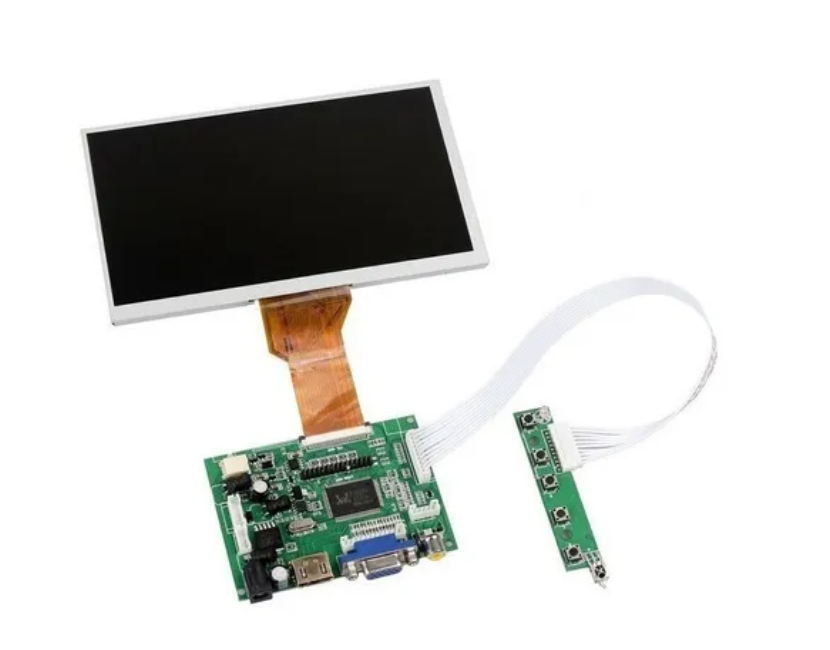
\includegraphics[scale=0.6]{figuras/TELAPI2.png}
  \caption{Tela da interface do usuário. }
  {\footnotesize Fonte : \cite{figura_Tela} } 
  \label{fig:Tela}
\end{figure}

\par Para a chegada dessa definição, pesquisas foram feitas e percebeu-se que geralmente telas menores, cinco e sete polegadas, possuem sensibilidade ao toque o que além de não agregar mais valor em nosso produto, dificultaria no dimensionamento da bateria dado a maior necessidade de potencia desse tipo de tela. Outro ponto levado em consideração é a questão da troca que existe entre o tamanho da tela e seu gasto energético. Precisava-se de uma tela grande o suficiente para a boa visualização dos dados, porém que fosse portátil e que consumisse pouca carga da bateria. Assim a escolha da tela com as características mencionadas anteriormente é justificada.

\par Para que o usuário interaja com essa tela, foi pensado em dois tipos de soluções. A primeira seria colocar todos os comandos em botões e chaves, e a segunda realizar os comandos por meio de um mini teclado. Optou-se pelo o uso do teclado, devido a possibilidade de maior interatividade com a aplicação de \textit{software} e facilidade para futuras atualizações no projeto. 

\par O modelo de teclado portátil escolhido pode ser visto na figura  \ref{fig:Teclado}. Esse teclado possui dimensões de 200x126x6,2 mm e um peso de 200g.





\begin{figure}[H]
  \centering
  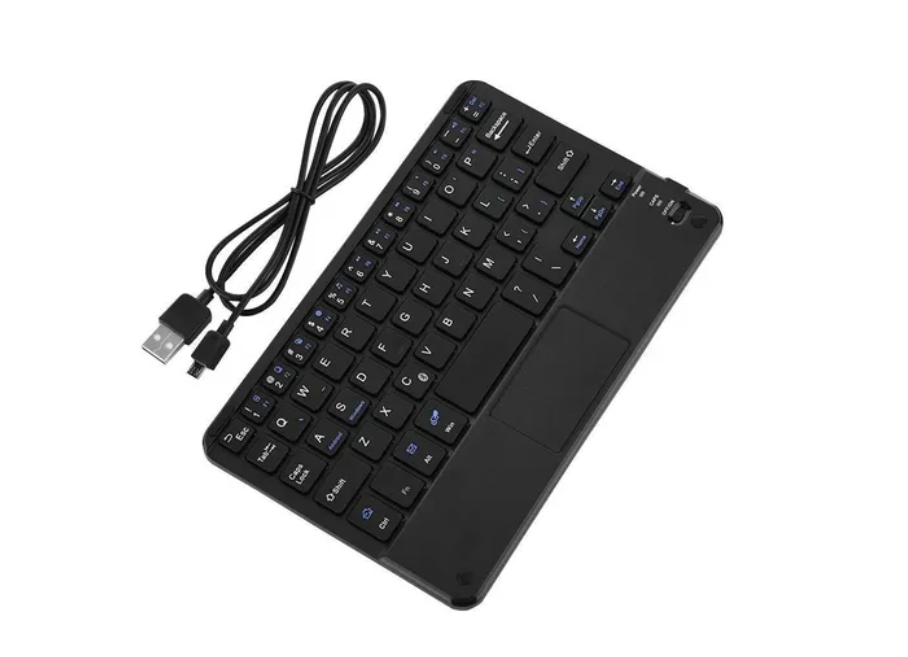
\includegraphics[scale=0.5]{figuras/TecladoPI2.png}
  \caption{Teclado da interface do usuário.}
  {\footnotesize Fonte : \cite{figura_Teclado}} 
  \label{fig:Teclado}
\end{figure}

\subsection{ \textit{Single Board Computer}}

\par Para a melhor escolha da placa utilizada no projeto, foi montada a seguinte tabela, na figura \ref{fig:comparacaoMicro}. Essa tabela foi levada aos grupos de \textit{software} e de energia para o debate entre capacidade de processamento e custo energético.

\begin{figure}[H]
  \centering
  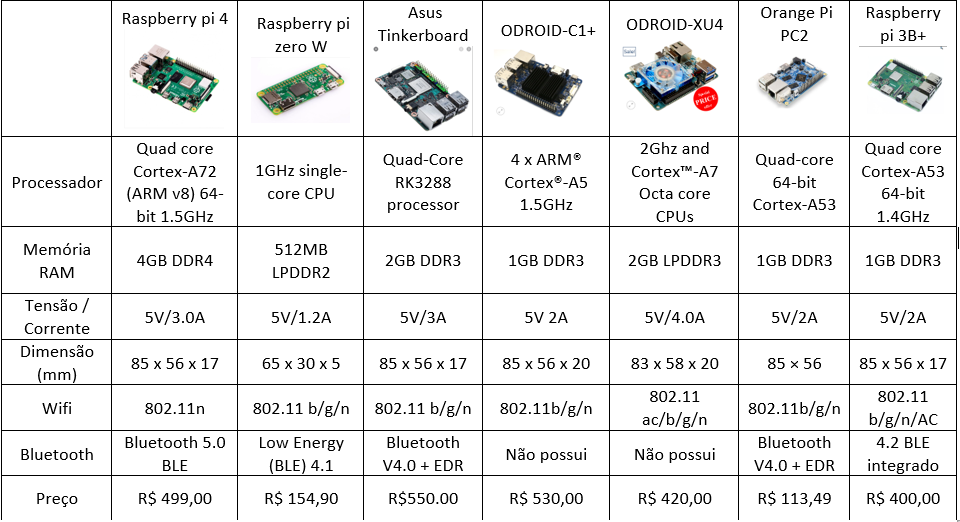
\includegraphics[scale=0.8]{figuras/SBCcomparacao.png}
  \caption{Tabela de comparação de \textit{single board computers}. Fonte : Autor } 
  \label{fig:comparacaoMicro}
\end{figure}

\par Após algumas reuniões, ficou decidido que se usaria a raspberry pi 3B+ no projeto. Porém, conforme as  \textit{sprints} foram passando, percebemos juntamente com o grupo de software que seria necessário mais capacidade de processamento para os algoritmos que seriam implementados. Um novo alinhamento geral foi feito e a escolha que melhor atenderia essa demanda de processamento seria o uso de uma Jetson Nano Developer Kit da Nvidia, mostrado na figura \ref{fig:Nvidea}. 

\begin{figure}[H]
  \centering
  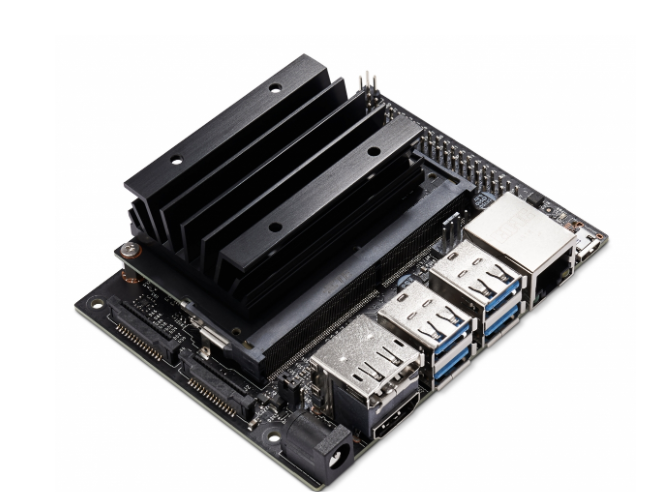
\includegraphics[scale=0.5]{figuras/NvideaPI2.png}
  \caption{Nvidea Jetson Nano Developer Kit. } 
  {\footnotesize Fonte : \cite{Nvidia_Nano} } 
  \label{fig:Nvidea}
\end{figure}

\par Apesar do detrimento causado no dimensionamento da bateria, essa placa foi escolhida devido a sua maior  capacidade de processamento de algoritmos mais pesados, assim suprindo a demanda encaminhada pela equipe de \textit{software}.

\par Juntamente com a equipe de energia foi construído um diagrama de blocos das interligações dos componentes, o mesmo pode ser visto  na figura \ref{fig:CentraldeCOntrole}. Visto as colaborações necessárias entre os dois grupos com relação ao dimensionamento da bateria, por parte da energia, e o consumo de potência de cada componente por parte da eletrônica. 


\begin{figure}[H]
  \centering
  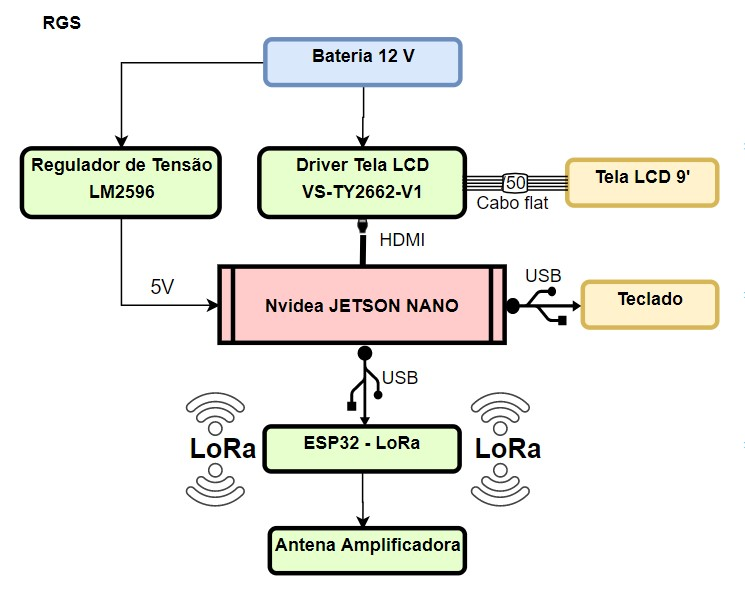
\includegraphics[scale=0.6]{figuras/Maleta_Diagrama.jpg}
  \caption{Diagrama Central de Controle. } 
  {\footnotesize Fonte : Autor } 
  \label{fig:CentraldeCOntrole}
\end{figure}

\section{Calibração}

\par Calibração é operação que estabelece, sob condições especificadas, num primeiro passo, uma relação entre os valores e as incertezas de medição fornecidos por padrões e as indicações correspondentes com as incertezas associadas; num segundo passo, utiliza esta informação para estabelecer uma relação visando a obtenção de um resultado de medição a partir de uma indicação. \cite{VIM_CALIBRACAO}.

\par Dentre os sensores utilizados na base de lançamento e no foguete, apenas as células de cargas da balança são transdutores necessários de calibração, os demais sensores já possuem calibração de fábrica, onde geralmente seus coeficientes de calibragem ficam armazenados em ROM.

\par Para calibrar a balança, após a montagem com as duas células de carga 50 Kg e o módulo conversor HX711, será executado uma rotina de ajuste do sistema de medição em código C no microcontrolador ESP32 LoRa. De acordo com o Vocabulário Internacional de Metrologia Legal (VIML) o ajuste de um sistema de medição é conjunto de operações efetuadas num sistema de medição, de modo que ele forneça indicações prescritas correspondentes a determinados valores de uma grandeza a ser medida. 

\par Através do programa executado deve ser encontrado um valor aferido  denominado como Fator de Ajuste para  ser inserido no programa de medição da Balança com o conversor, e assim a calibração seja realizada.

\par O programa de ajuste fará uso da biblioteca \href{https://github.com/bogde/HX711}{HX711.h}, onde um objeto de peso conhecido deve ser lido pela balança, e a média dos valores retornados deve ser dividido pelo valor do peso real do objeto em KG, obtendo o fator de ajuste, que deve ser inserido como parâmetro da função “scale.set\textunderscore scale()” importada da biblioteca mencionada. Com esse fator de ajuste setado, obtém-se a calibração da balança, medindo então o do peso real do objeto \cite{CALIBRACAO_tutorial}.

\par A figura \ref{fig:Calibracao_balanca} apresenta o fluxograma do algoritmo de ajuste e calibração dos sensores da balança.

\begin{figure}[H]
  \centering
  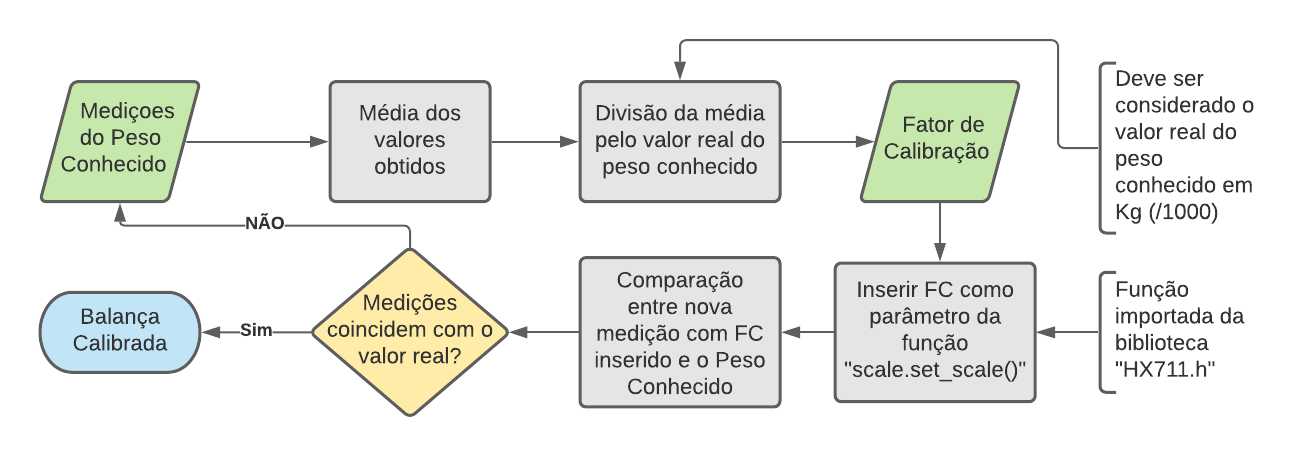
\includegraphics[scale=0.6]{figuras/Algoritmo de Calibração da Balança.png}
  \caption{Diagrama do algoritmo de calibração da balança } 
  {\footnotesize Fonte : Autor } 
  \label{fig:Calibracao_balanca}
\end{figure}

Convém ressaltar que foi escolhido para os dados de peso medidos pela balança, uma precisão de 3 casas decimais. Esta precisão é definida como um parâmetro setado em uma função contida na biblioteca \href{https://github.com/bogde/HX711}{HX711.h}.

\section{Integrações}
\subsection{Diagrama de blocos do Abastecimento}
\par Apos reuniões com a equipe de estrutura e com a CRT, foram levantados os requisitos para o abastecimento do foguete de forma mais especifica. Foi criado um diagrama lógico para melhor entendimento do procedimento, figura \ref{fig:Abastecimento do fohuete}, maiores detalhes estão apresentados no capitulo \ref{abastecimento}. Assim, foi possível a equipe estrutural definir quais motores se enquadram para cada válvula do sistema.
\par É necessário um conjunto de 3 motores para a parte externa do foguete, um para a válvula 1 responsável por abrir o cilindro do combustível, um para a válvula 2 que é responsável por despressurizar a mangueira após a conclusão do abastecimento,um para o desacoplamento do engate rápido e o ultimo para o acionamento da ignição, sendo que estes dois ultimos seriam acionados por um modulo de dois relés SRD‑05VDC‑SL‑C, por necessitarem se movimentarem somente em uma direção linear tanto no desengate quanto na ignição, diferentemente dos outros dois citados anteriormente, que necessitam se movimentarem nos dois sentidos (horário e anti-horário, para abertura e fechamento das válvulas), fazendo-se necessário usar o modulo L298N, que é uma ponte H dupla.  
\par Já na parte interna do foguete, existem dois atuadores, que seriam acionados também de modo remoto: a válvula 4, que é uma válvula solenoide, responsável pelo controle da pressão do tanque do foguete, ou seja, ela fica abrindo e fechando a fim de estabilizar a pressão interna do foguete liberando gases internos durante o abastecimento; e a válvula 5, que é aberta na ignição, expulsando o óxido nitroso do tanque do foguete em direção à câmara de combustão. Ambas serão abertas em um só sentido; portanto, foi proposto usar um módulo de dois relés SRD‑05VDC‑SL‑C para seu acionamento pelo microcontrolador interno do foguete.
     


\begin{figure}[H]
  \centering
  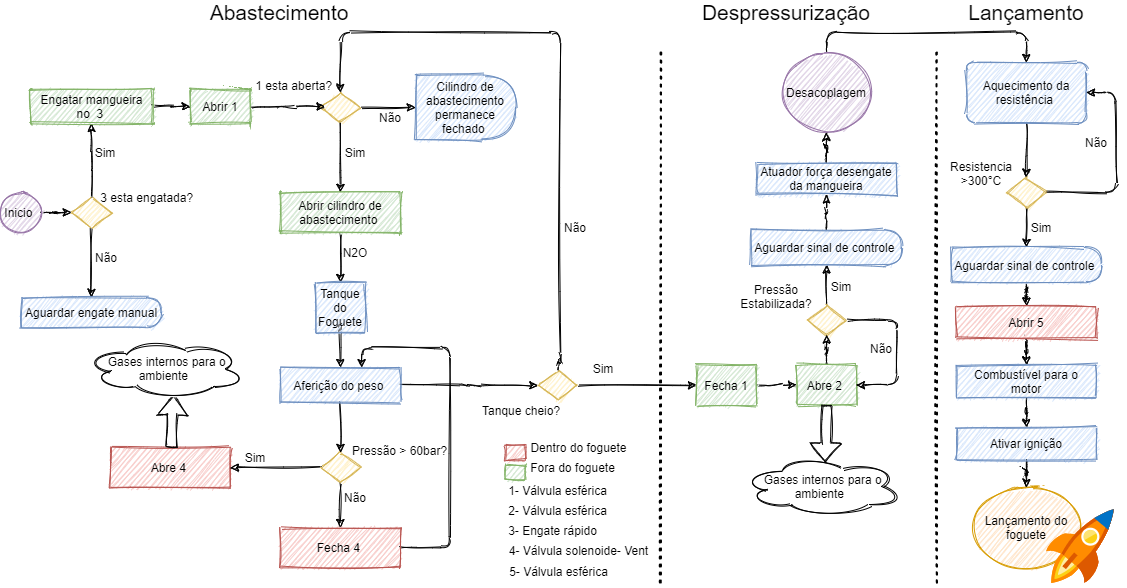
\includegraphics[scale=0.35]{figuras/abastecimento .png}
  \caption{ \href{https://drive.google.com/file/d/1EhMWyoD2Ml5I2vsLA0MbNOR8LxuCMmC5/view?usp=sharing}{ Diagrama logico do abastecimento foguete}. } 
  {\footnotesize Fonte : Autor } 
  \label{fig:Abastecimento do fohuete}
\end{figure}

\subsection{Acionamento eletrônico das válvulas externas e ignição}

\par As válvulas externas terão o seu acionamento controlado pelo microcontrolador ESP32 LoRa contido na base de lançamento do foguete, o qual também atua no controle da balança. Por meio dele serão enviados comandos de acionamento para fechar e abrir as válvulas externas durante o processo de abastecimento do foguete.

\par De acordo com informações obtidas do grupo de estrutura, serão necessários 3 adaptadores externos, sendo 2 válvulas esféricas que atuam no tanque de combustível e mangueira, e 1 atuador para desengate rápido, onde é necessário apenas o desengate remoto, pois o engate é manual. 

\par As válvulas esferas serão acionadas por meio de dois motores, um para cada válvula, onde o microcontrolador fará o seu acionamento por meio de uma Ponte H, enviando comandos para girar o motor em sentido horário ou anti-horário, ou seja, abrir ou fechar a válvula. A solução mecânica entre motores e válvulas é detalhado na estrutura.

\par De acordo com a estrutura, os motores usados para controle das válvulas esferas são do modelo Mabuchi 8d 12V. Esse motor é alimentado com 12V, com um consumo de corrente de 1,3A e torque de 9,12 N.m / 93 Kg. Para controle dos motores será necessário o uso de ponte H para realizar abertura e fechamento, controlando o sentido de rotação dos motores. 

\par A ponte H é um circuito que serve para variar o sentido da corrente em uma determinada carga, bem como controlar sua potência. A figura \ref{fig:PonteH_circuito} apresenta o circuito típico de uma ponte H.

\begin{figure}[H]
  \centering
  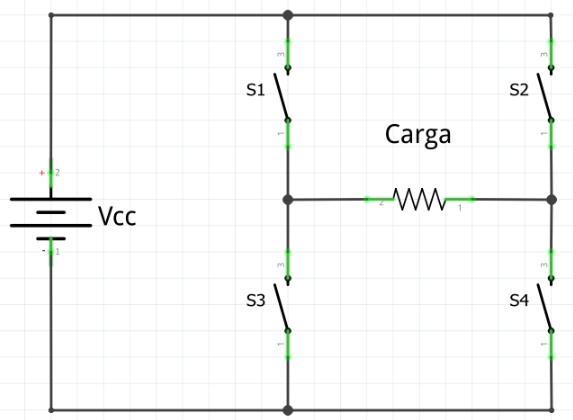
\includegraphics[scale=0.3]{figuras/ponteH_circuito.png}
  \caption{ Circuito típico de uma ponte H.} 
  {\footnotesize Fonte : \cite{PonteH_Teoria}} 
  \label{fig:PonteH_circuito}
\end{figure}

\par Com base nas especificações dos motores, foi escolhido o Driver Motor Ponte H L298n, figura \ref{fig:PonteH_modulo}, para controle destes. Esse módulo possui tensão de operação de 4 a 35V, com corrente de operação máxima de 2A por canal (ou 4A máxima), tensão lógica de 5V, corrente lógica de 0 a 36mA e potência máxima de 25W \cite{PonteH_Datasheet}. O grande benefício desse módulo é que, com ele, é possível controlar dois motores ao mesmo tempo e, se necessário, controlar a velocidade deles, atuando no PWM do sinal enviado.

\begin{figure}[H]
  \centering
  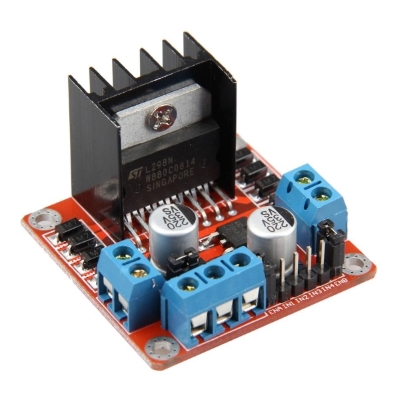
\includegraphics[scale=0.4]{figuras/ponteH_modulo.jpg}
  \caption{ Driver Motor Ponte H L298n.} 
  {\footnotesize Fonte : \cite{PonteH_mod}} 
  \label{fig:PonteH_modulo}
\end{figure}

\par Como o módulo da ponte H trabalha com tensão lógica de 5V, é necessário o uso de um conversor lógico de 3.3V (tensão lógica dos pinos da ESP32 LoRa) para 5V. Para tal, foi escolhido o Módulo Conversor Nível Lógico 5V/3.3V - Bidirecional (4 Canais), figura \ref{fig:CONV_LOGICO}. Esse conversor é capaz de elevar tensões de nível lógico de 3,3V para 5V, e isso de forma totalmente segura, possuindo 4 canais independentes que permitem a conversão de sinal. Entretanto, o conversor não é capaz de funcionar com sinais analógicos. A placa necessita de alimentação das duas tensões (alta tensão e baixa tensão) com que seu sistema estiver trabalhando \cite{Conversor_logico}.

\begin{figure}[H]
  \centering
  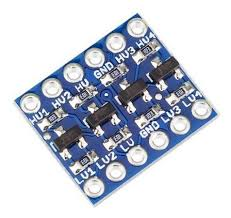
\includegraphics[scale=0.4]{figuras/conv_logico.jpeg}
  \caption{ Módulo Conversor Nível Lógico 5V/3.3V - Bidirecional (4 Canais)} 
  {\footnotesize Fonte : \cite{Conv_logico}} 
  \label{fig:CONV_LOGICO}
\end{figure}

\par Ressalta-se que na parte externa ao foguete, tem-se também o engate rápido, cuja solução mecânica não faz parte do escopo do projeto e sim da CRT. Todavia, apenas o acionamento eletrônico do seu desacoplamento do foguete faz parte do escopo da eletrônica, devido a necessidade de fazê-lo de maneira remota. 

\par Para tal, a solução adotada pela CRT é que o desacoplamento do engate seja feito com o auxílio de um motor de vidro elétrico universal, modelo Mabuchi 8d 12v, o mesmo modelo utilizado para as válvulas esferas. O desacoplamento deve ocorrer quando o motor for acionado, onde um cabo de aço preso ao engate irá enrolar ao eixo no motor, puxando a mangueira para fora do engate.

\par Por fim, tem-se externo ao foguete a resistência de ignição, um fio ignitor de Níquel Cromo (Ni-Cr) com resistência calculada em 2,23 Ohms, a qual deve ser acionada pelo microcontrolador da base, assim que o comando for enviado para propulsão do foguete. O acionamento da ignição é realizado quando uma corrente de 5,38A passa pela resistência, alimentada pela bateria de 12V e esta encandeia alcançando a temperatura de 300°C, fazendo o propelente entrar em combustão.

\par Uma vez que o motor de desengate não precisará inverter o sentido de rotação, e a resistência de ignição é acionada pela passagem de uma corrente direta, ou seja, tensão DC; não é necessário o uso de ponte H, portanto, para realizar ambos acionamentos, será utilizado um módulo  Módulo Relé 5V 2 Canais modelo SRD-05VDC-SL-C, figura \ref{fig:RELE_2CHANNEL}. Esse relé possui 2 canais, um para o motor de desengate e outro para a resistência de ignição, possui tensão de operação de 5V, com um consumo de corrente típica de 15~20mA e possui capacidade na faixa de (30 VDC a 10A) ou (250VAC a 10A), o que atende a especificação do motor Mabuchi e da resistência de ignição \cite{rele_two}.

\begin{figure}[H]
  \centering
  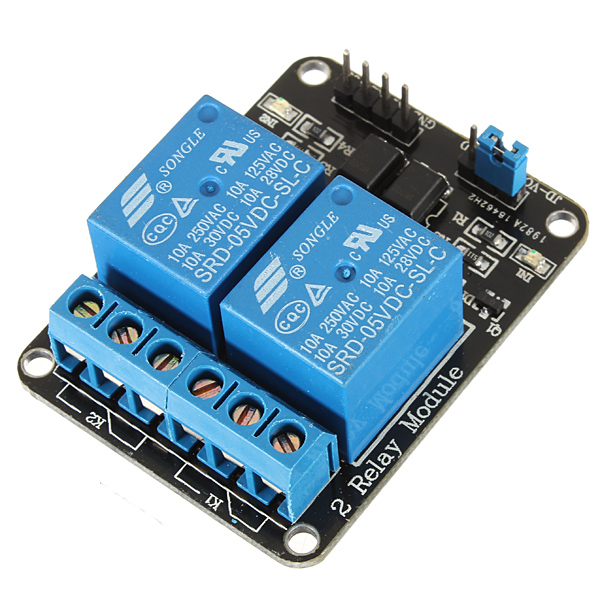
\includegraphics[scale=0.3]{figuras/RELE_2CHANNEL.jpg}
  \caption{ Módulo Relé 5V 2 Canais modelo SRD-05VDC-SL-C} 
  {\footnotesize Fonte : \cite{rele_photo}} 
  \label{fig:RELE_2CHANNEL}
\end{figure}

\par A conexão dos módulos atuadores das válvulas, do desengate e da ignição no microcontrolador é estabelecido conforme esquema da figura \ref{fig:base_valvulas}.

\begin{figure}[H]
  \centering
  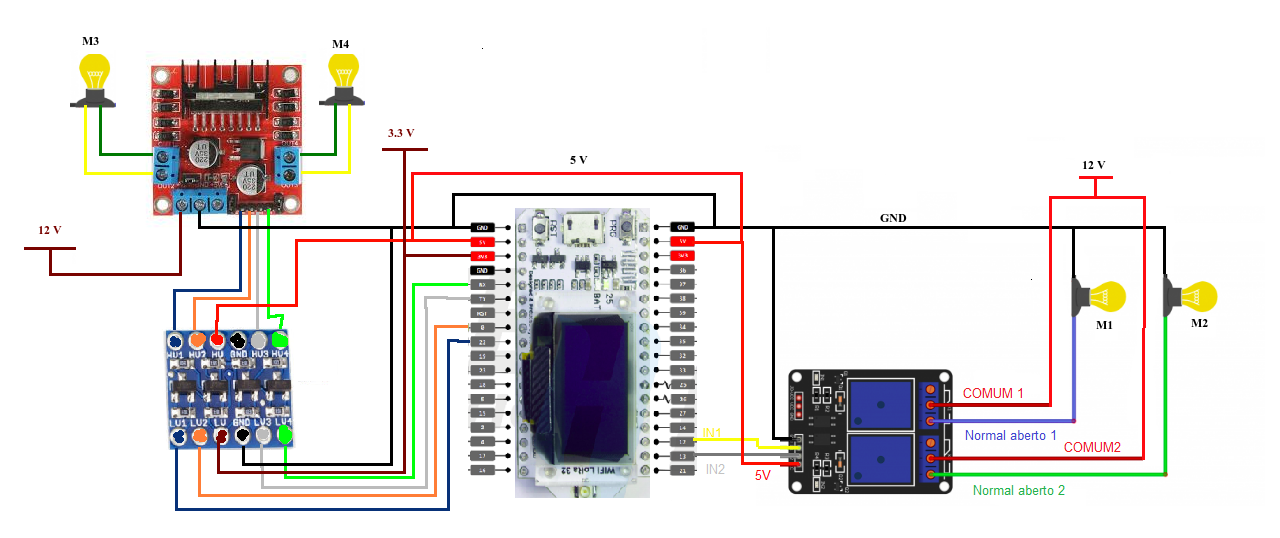
\includegraphics[scale=0.5]{figuras/BASE_VALVULAS.png}
  \caption{ Conexões entre atuadores externos e microcontrolador da base de lançamento. } 
  {\footnotesize Fonte : Autor}
  \label{fig:base_valvulas}
\end{figure}

\par Onde, M1 é o motor do desengate remoto, M2 é a resistência de ignição e M3 e M4 são os motores de abertura e fechamento das válvulas esferas do cilindro de combustível e mangueira, respectivamente.

\subsection{Acionamento eletrônico das válvulas internas}

\par As válvulas internas do foguete, serão controladas e acionadas pelo microcontrolador ESP32 LoRa presente no foguete, o qual também faz o controle dos sensores de pressão e temperatura e módulo GPS.

\par Uma vez que é necessário acionar com precisão a válvula 4, ou seja, uma válvula solenoide, não é necessário o uso de ponte H. Portanto, para realizar o acionamento desta, será utilizado um relé que atende a necessidade de ficar acionando a válvula solenoide de tempo em tempos, e a outra válvula interna é do tipo esférica que será aberta somente uma vez também será acionado por relé,assim foi definido o uso do Módulo Relé 5V 2 Canais modelo SRD-05VDC-SL-C, figura \ref{fig:RELE_2CHANNEL}, com as configurações supracitadas anteriormente. Esse relé possui 2 canais, um para a válvula solenoide e um para o motor da válvula 5 controlados pela ESP32-LoRa de dentro do foguete que mandará os sinais de controle para o modulo de relés e pode ser observado melhor no diagrama esquemático do circuito interno do foguete na figura \ref{fig:Diagrama esquematico do circuito interno do foguete}.

\subsection{Comunicação hardware e software}

\par Visto que um dos maiores objetivos do projeto é a realização da telemetria com os dados vindos do foguete,este tópico tratará a maneira pela qual será realizada a comunicação entre o \textit{hardware} e a aplicação de \textit{software} e também como o dado trafegará em todo o sistema.

\par Para exemplificar de forma mais clara o caminho e os protocolos usados, a explicação será feita pro meio do apêndice \ref{diagrama_sequencia}, onde juntamente com a equipe de \textit{software} foi desenvolvido um diagrama de sequência tratando os processos que envolvem esta comunicação.


%\begin{figure}[H]
%  \centering
%  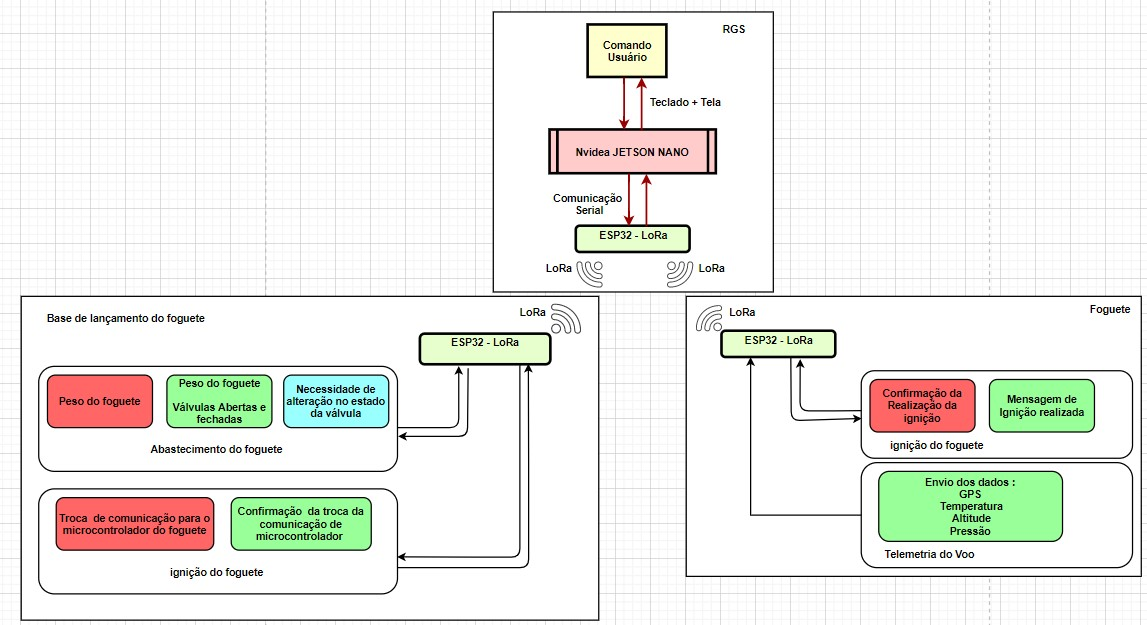
\includegraphics[scale=0.7]{figuras/Fluxo_dados.jpg}
%  \caption{ Fluxo de dados} 
%  {\footnotesize Fonte : Autor} 
%  \label{fig:FLuxoDados}
%\end{figure}

\par Todos os comandos são inseridos pelo usuário por meio do teclado, então o \textit{software} do sistema informa essas ações via comunicação serial para o microcontrolador da maleta, pois ambos estão conectados via USB. Assim que o comando chegar neste primeiro microcontrolador, ele é transmitido para a base do foguete ou para o próprio foguete, via comunicação LoRa, dependendo do processo que esta sendo executado.

A partir do momento em que a missão de lançamento é iniciada pelo usuário figura \ref{fig:Diagrama_sequencia_missao}, sera estabelecido uma comunicação entre os microcontroladores da maleta e da base, esta comunicação durará até a faze da ignição do foguete. Com essa comunicação estabelecida o primeiro comando a ser executado é do abastecimento do foguete \ref{fig:Diagrama_sequencia_abastecimento}. Para este comando é necessário que sejam enviados os dados do peso do foguete vazio e o peso do foguete cheio, assim que esses dados forem inseridos eles serão transmitidos para o microcontrolador da base e uma confirmação de inicio de abastecimento será retornada. Durante o abastecimento o dado do peso atual do foguete será transmitido para a interface do usuário até que peso esperado seja atingido, quando uma confirmação será enviada indicando o termino do processo.

O próximo comando é o do desengate da mangueira de abastecimento figura \ref{fig:Diagrama_sequencia_desengate}. Assim que este comando for aplicado pelo usuário, uma confirmação de inicio de desengate será retornada do hardware para o software e, como dito anteriormente, o comando será enviado para o microcontrolador da base, que executará  a despressurização da mangueira e posteriormente o acionamento do motor responsável pelo  desengate.Após o processo uma confirmação de termino do desengate será retornada.

Seguindo o processo, o próximo comando trata-se do inicio da ignição e é durante este comando em que ocorre a troca de comunicação do sistema da base para o o microcontrolador do foguete. Assim que este comando é acionado o microcontrolador da base aciona o ignitor e a troca da comunicação, citada anteriormente, é realizada. A partir do momento em que a comunicação com o foguete for estabelecida a válvula de lançamento será aberta, fazendo com que o foguete seja lançado.A partir deste momento o usuário receberá uma mensagem de termino da ignição e passará a receber todas as informações dos sensores do foguete.  







\section{Diagramas e esquemáticos}

\par Com a definição da solução e dos componentes da base de lançamento, foi criado o esquemático do circuito integrado, com detalhamento de pinos, conexões e módulos utilizados. A figura \ref{fig:Diagrama esquematico do circuito interno da base de lancamento} apresenta o circuito integrado da base de lançamento, com os componentes da balança e os módulos dos atuadores externos, assim como bornes para os motores. Na figura \ref{fig:Diagrama esquematico do circuito interno do foguete}, encontra-se o diagrama esquemático, o detalhamento das conexões do sensoriamento interno do foguete, assim como a parte de controle das válvulas internas. Na figura \ref{fig:Diagrama esquemático do circuito da central de controle do usuário}, por sua vez, tem-se o esquemático com as conexões na base central de comando entre a ESP32 Wifi Lora e a Jetson e outros periféricos. Os esquemáticos foram feitos utilizando as ferramentas do \textit{software} EasyEDA ,assim como o projeto de suas PCIs.

\begin{figure}[H]
  \centering
  \includegraphics[scale=0.35]{figuras/PDFs/final eletronica/Schematic_base de lançamento.pdf}
  \caption{Diagrama esquemático do circuito interno da base de lançamento.} 
  {\footnotesize Fonte:Autor} 
  \label{fig:Diagrama esquematico do circuito interno da base de lancamento}
\end{figure}

\begin{figure}[H]
  \centering
  \includegraphics[scale=0.35]{figuras/PDFs/final eletronica/Schematic_Esquemático foguete.pdf}
  \caption{Diagrama esquemático do circuito interno do foguete. } 
  {\footnotesize Fonte:Autor} 
  \label{fig:Diagrama esquematico do circuito interno do foguete}
\end{figure}

\begin{figure}[H]
  \centering
  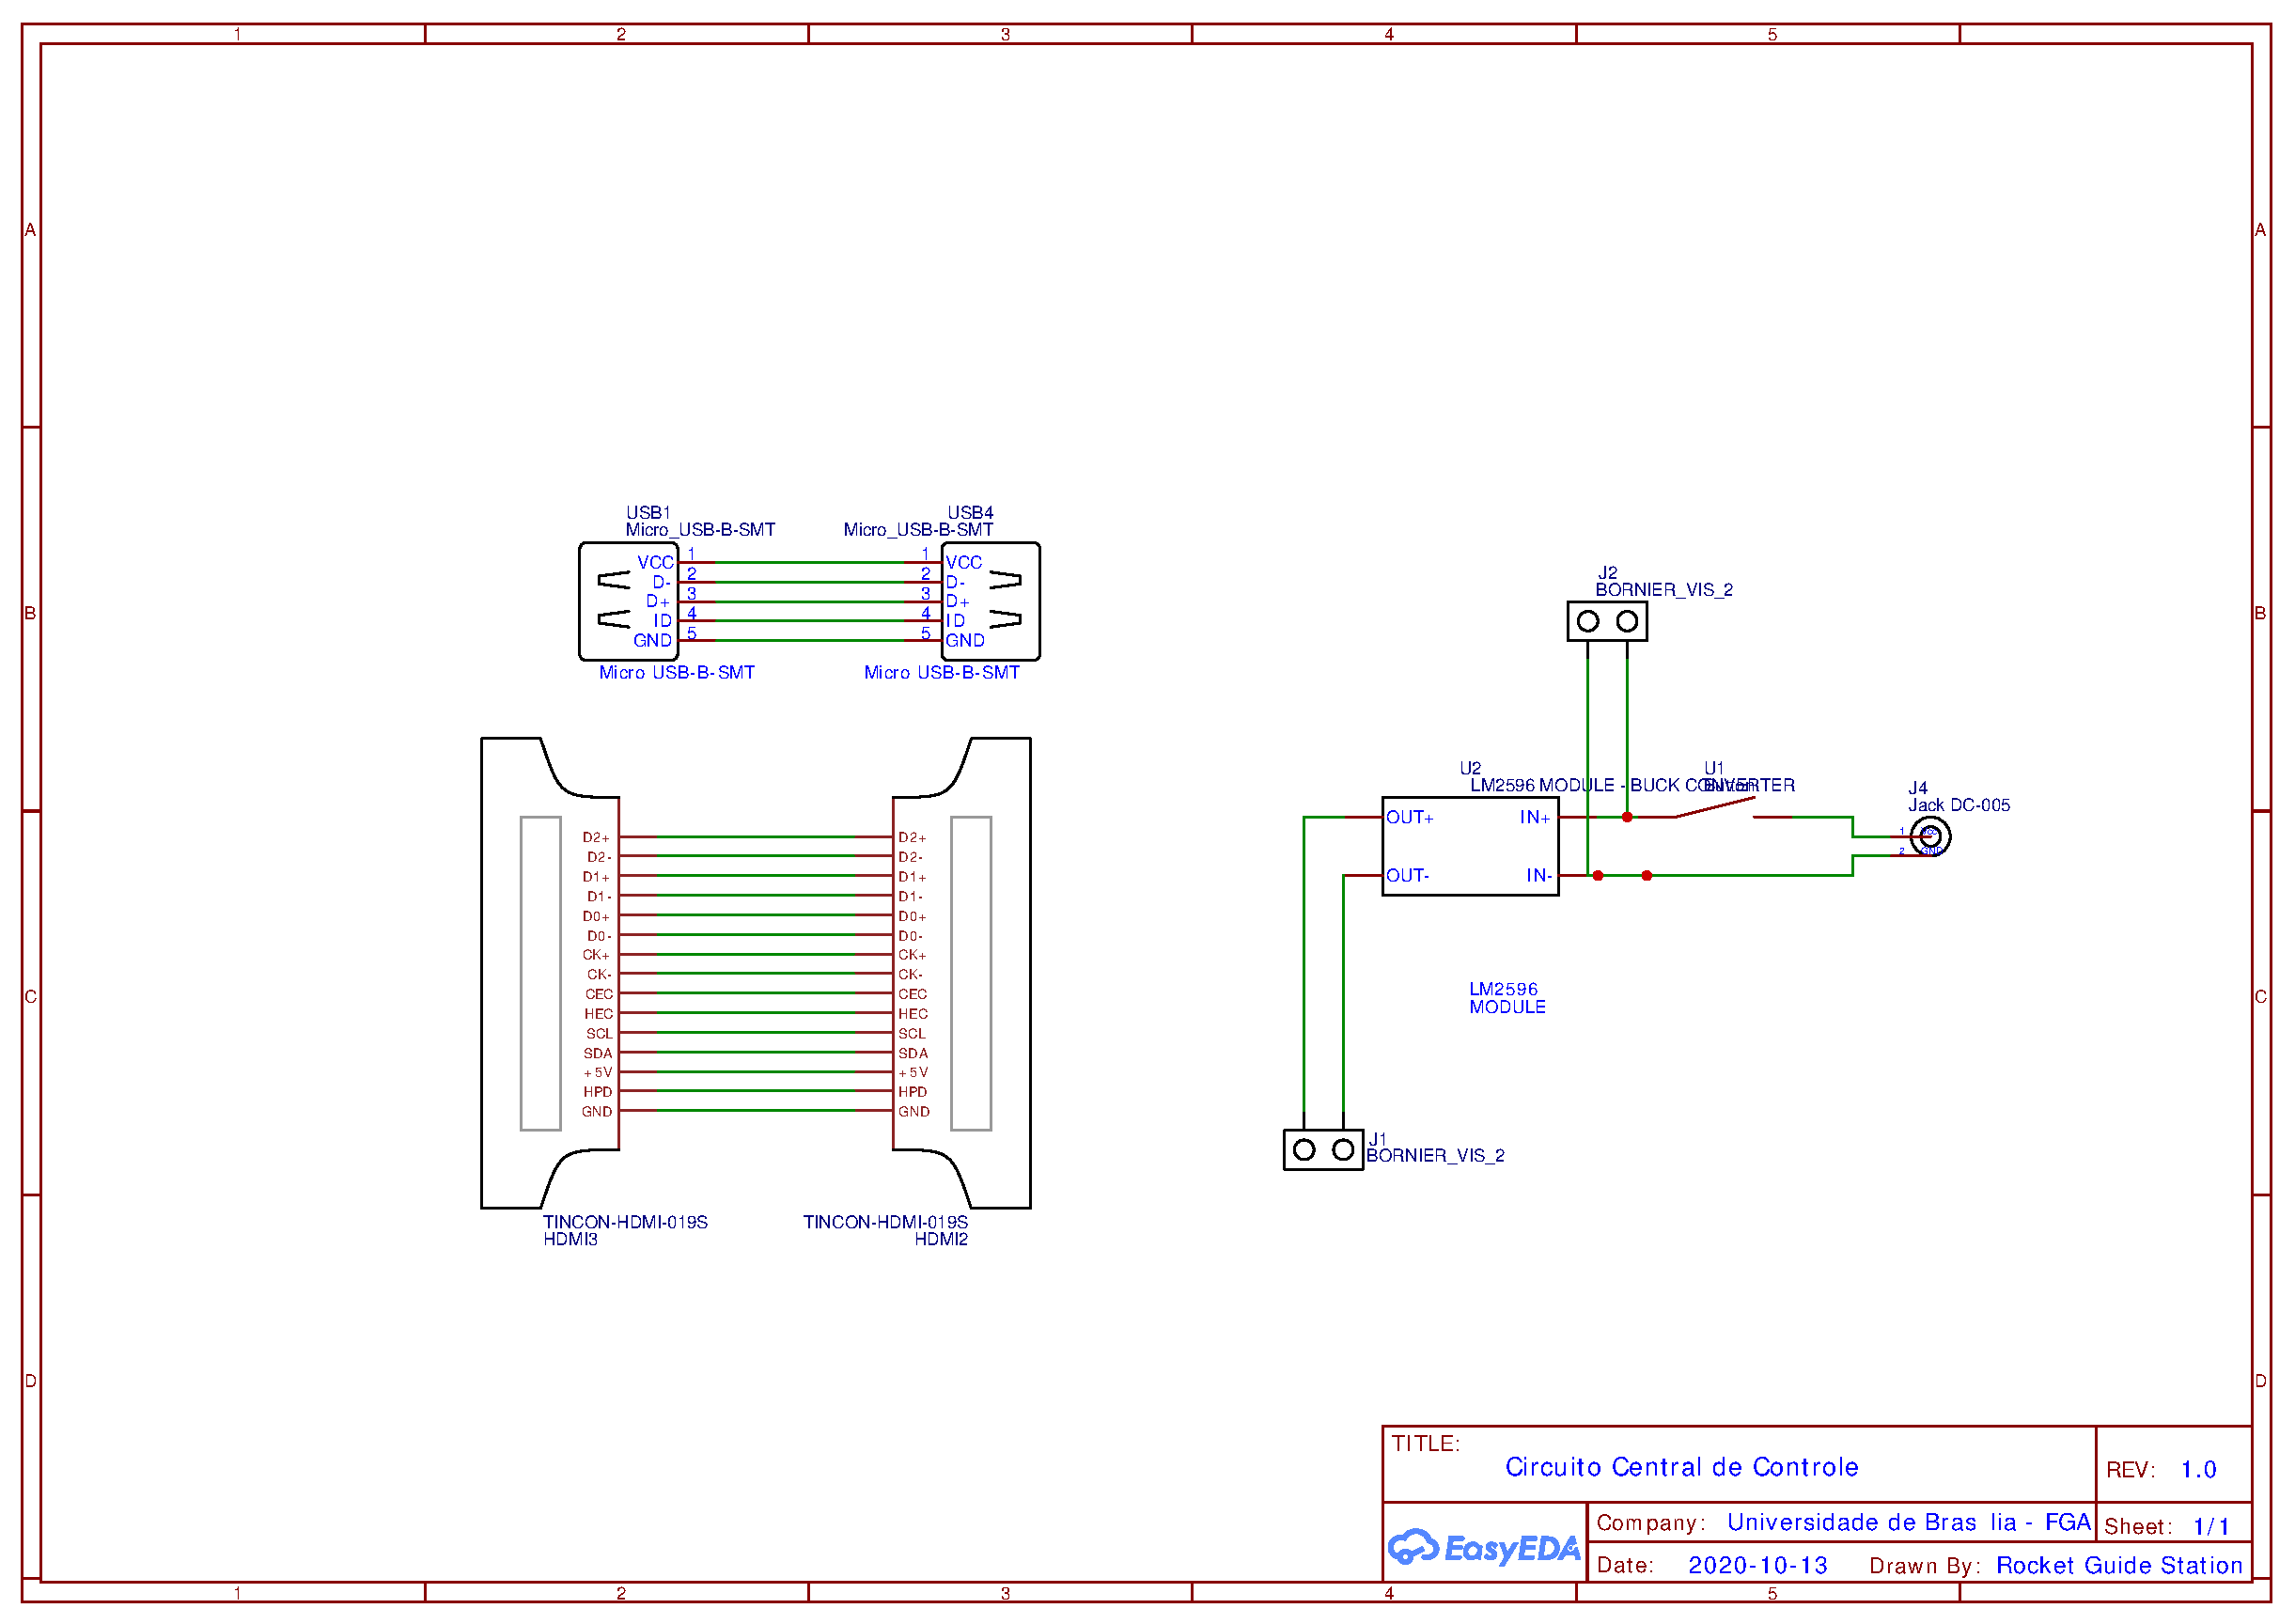
\includegraphics[scale=0.35]{figuras/PDFs/final eletronica/Schematic_maleta final.pdf}
  \caption{Diagrama esquemático do circuito da central de controle do usuário.} 
  {\footnotesize Fonte:Autor} 
  \label{fig:Diagrama esquemático do circuito da central de controle do usuário}
\end{figure}

\section{Placa de circuito impresso}

\par Para melhor funcionamento  e durabilidade do circuito, é necessária a criação do desenho de placa de circuito impresso, conhecido como PCI, que é gerido por regras que visam garantir a qualidade do funcionamento do circuito IPC-2221B \cite{IPC-2221}, visando a disposição dos componentes para melhor acomodação mecânica e eletromagnética, a fim de evitar interferências no circuito.
\par Basicamente, é constituída por uma base de um material isolante, geralmente fenolite ou fibra de vidro, revestida por uma fina camada de cobre na sua superfície, onde ocorre as ligações entres os componente eletrônicos que podem ser do tipo PTH ou SMD\cite{pci}. 

\par As placas utilizadas nesse projeto serão feitas de modo a acomodar componentes do tipo PTH, ou seja, componentes que serão inseridos na placa através de um furo denominado de pads, sendo necessário uma acurácia para não errar no distanciamento dos furos, evitando assim mal posicionamento dos componentes eletrônicos.
\par Outro levantamento importante que é necessário fazer no projeto de uma PCI é a largura das trilha, que são responsáveis pelas conexões elétricas entre os componentes, a qual é determinada pela corrente que irá passar pela trilha e pela espessura da trilha de cobre  e a temperatura \cite{ TecnicasdeProjetosPCI}. Os cálculos das trilhas foram feitos no site \href{https://pcbbrasil.com.br/calculo-trilha-pcb.php}{PCBBRASIL} que segue os critérios da norma IPC-2221B para confecção de placas de circuito impresso.
\par Para a confecção da placa de circuito impresso foi gerado o arquivo Gerber de cada placa de circuito impresso, sendo gerado um arquivo em formato ZIP disponível em \href{https://drive.google.com/drive/folders/1P1pQGE_zuSLOB5qd8zfESWqLDwtyoRKd?usp=sharing}{ Arquivos Gerber}. Para a visualização dos arquivos Gerber é necessário a utilização de um programa de prototipagem de placas de circuito impresso ou um visualizador desse tipo de arquivo disponível para \href{https://sourceforge.net/projects/gerbv/files/}{ \textbf{download}} no site do programa utilizado para o projeto EasyEda.

\subsection{Circuito interno do foguete}
\par Na figura \ref{fig:Diagrama esquematico do circuito interno do foguete}, está representado o circuito interno do foguete. Assim, na figura \ref{fig:PCIFOGUETE}, encontra-se o  projeto mecânico da placa de circuito impresso com as dimensões para sua fabricação. Foram adicionados cinco buracos na PCI no intuito de facilitar sua fixação dentro do foguete com parafusos de diâmetro de 5mm. Na figura \ref{fig:PCB_FOGUETE}, por sua vez, é apresentado o modelo 3D da PCI com com o sistema de alimentação à esquerda da placa, separado dos outros componentes a fim de evitar interferência eletromagnética no restante da placa. Foi adicionado a essa placa esse sistema para garantir a tensão adequada para os componentes. 
\par A placa a ser produzida possui espessura padrão de 1,6mm, com tolerância nominal de $\frac{+}{-}$ 0,13mm. Nessa PCB específica, são utilizadas duas camadas de cobre para as trilhas; portanto, serão feitas trilhas tanto na \textit{Top Layer} quanto na \textit{Bottom Layer}, ou seja, \textit{multilayer}, garantindo uma melhor distribuição das trilhas. Por ser um módulo que vai dentro do foguete, inicialmente foi pensado em usar componentes do tipo PTH e a plaquinha de desenvolvimento da ESP32Lora, da Heltec, pois não são feitos muitos lançamentos. A ideia é utilizar primeiramente uma PCB nesse formato para testes e melhorias no projeto, antes de confeccionar uma placa mais enxuta com componentes SMD. 
\par Para essa versão inicial das placas de circuito impresso, seriam feitas de fenolite (FR2), que é um material mais barato para a confecção e quando tiver os componentes testados será feito em material de vibra de vidro(FR4)\cite{CONCEITOpci}.

\begin{figure}[H]
  \centering
  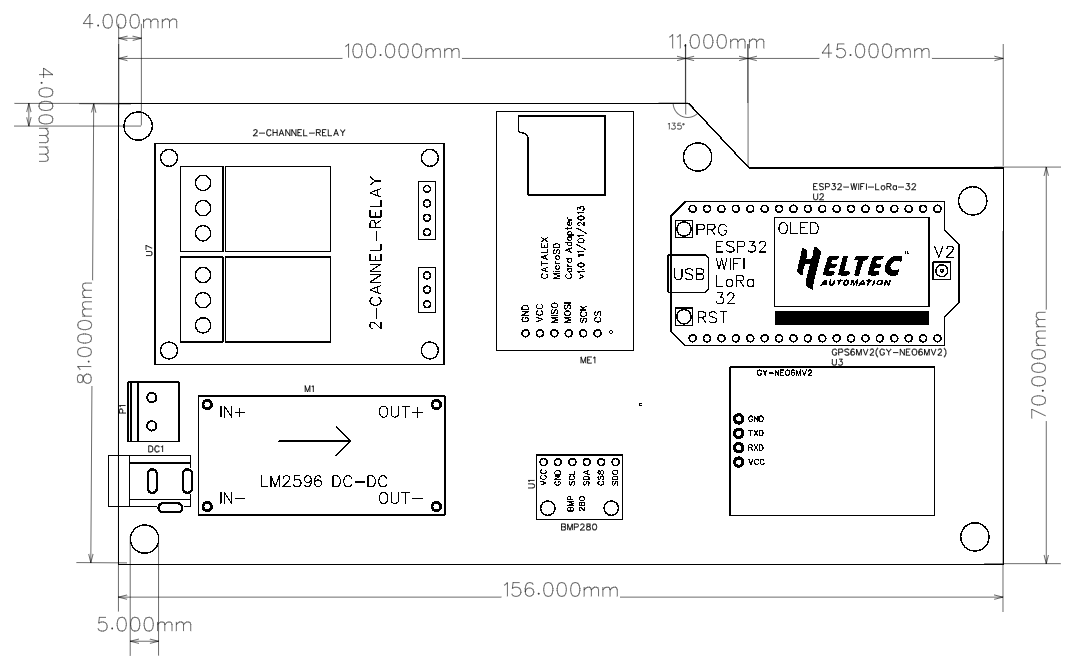
\includegraphics[width=\textwidth]{figuras/PDFs/final eletronica/PCB_PCB_interna do foguete.png}
  \caption{Dimensões da PCI do circuito interno do foguete.} 
  {\footnotesize Fonte : Autor } 
  \label{fig:PCIFOGUETE}
\end{figure}

\begin{figure}[H]
  \centering
  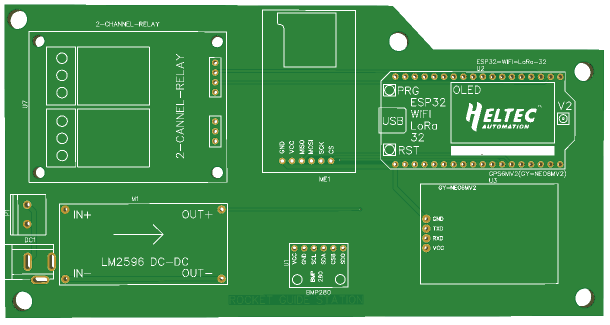
\includegraphics[scale=0.4]{figuras/PDFs/final eletronica/foguete_top.png}.
    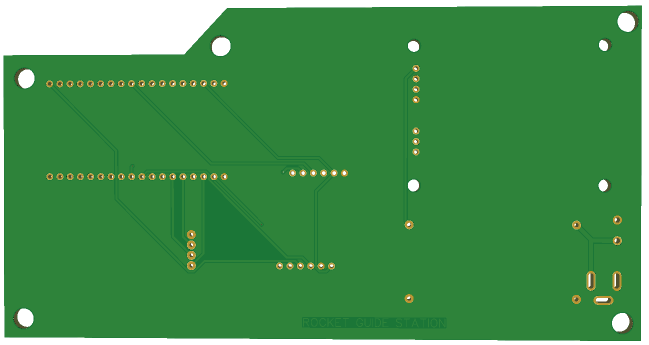
\includegraphics[scale=0.4]{figuras/PDFs/final eletronica/foguete_bottom.png}
  \caption{PCI do circuito interno do foguete.} 
  {\footnotesize Fonte : Autor } 
  \label{fig:PCB_FOGUETE}
\end{figure}


\subsection{Circuito na base de lançamento}
\label{sec:base_de_lancamento}

Objetivando reduzir o número de fios e cabos utilizados no circuito da base de lançamento, assim como obter a menor ocupação de volume de circuitaria e componentes, foi criado o modelo de PCI com base no circuito integrado citado na figura \ref{fig:Diagrama esquematico do circuito interno da base de lancamento}. Foi optado o modelo \textit{Bottom Layer} para as trilhas da PCI, ou seja, contém apenas uma camada de cobre.

A figura \ref{fig:PCB_BASE_LANCAMENTO_DES} mostra o desenho da PCI, junto com suas cotas de dimensões definidas, que foram de 88mm x 109mm. Os buracos nos cantos da PCB, com diâmetro de 4mm e distâncias das bordas de 3mm, servem pra fixação da placa na estrutura da base.

\begin{figure}[H]
  \centering
  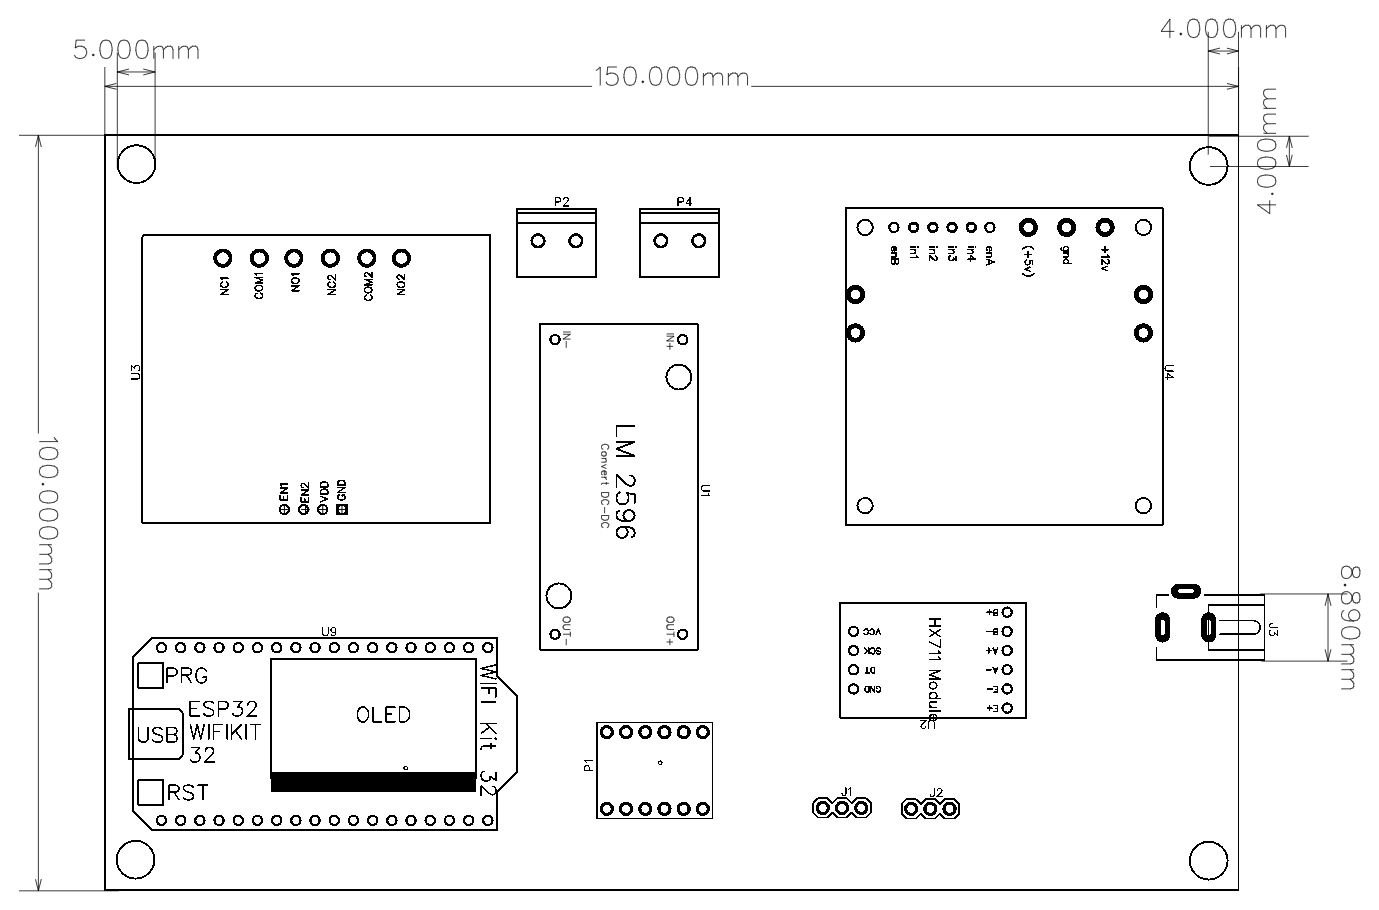
\includegraphics[width=\textwidth]{figuras/PDFs/final eletronica/PCB_BASE_FINAL.png}
  \caption{ Dimensões da PCI do circuito interno da base de lançamento. } 
  {\footnotesize Fonte : Autor } 
  \label{fig:PCB_BASE_LANCAMENTO_DES}
\end{figure}

A figura \ref{fig:PCB_BASE_LANCAMENTO} apresenta a visão frontal da PCI, onde é possível visualizar a posição dos componentes, tais como encaixes dos pinos e os bornes dispostos nas extremidades, e a visão traseira da PCI, onde se encontra a camada de fundo (\textit{Bottom Layer}), com as trilhas do circuito.

\begin{figure}[H]
  \centering
  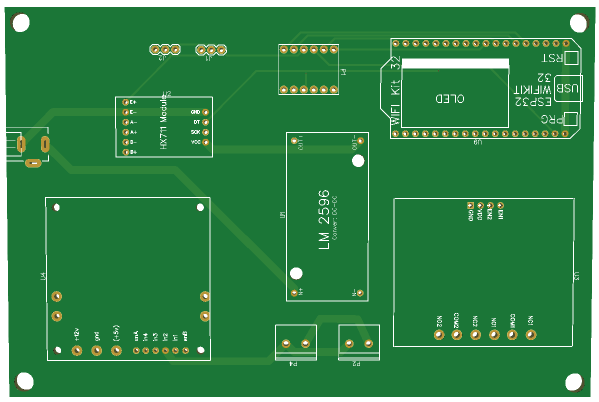
\includegraphics[scale=0.4]{figuras/PDFs/final eletronica/BASE_TOP.png}
    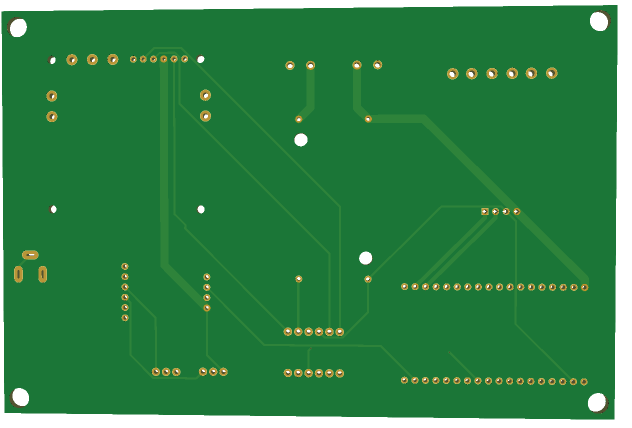
\includegraphics[scale=0.4]{figuras/PDFs/final eletronica/BASE_BOTTOM.png}
  \caption{PCI do circuito interno da base de lançamento } 
  {\footnotesize Fonte : Autor } 
  \label{fig:PCB_BASE_LANCAMENTO}
\end{figure}

\subsection{Circuito na base de controle central}

A ideia dessa PCI é reduzir o número de cabos utilizados dentro da maleta do usuário.
De acordo com o espaço e a disposição dos componentes mostrado na figura  \ref{fig:Disposicao dos Componentes} e na figura \ref{fig:PCB_controle} pensou-se em fazer uma placa de modo que os módulos sejam encaixados nas laterais da PCI. Para isso foi verificado todos desenhos técnicos dos componentes, mapeando então os conectores  por meio dessas medidas fornecidas pelo fabricante. Os conectores precisarão ser do tipo macho para que o encaixe seja realizado. Isso traz vantagens: caso algum módulo sofra dano, bastará  desconectá-lo e realizar a troca.

\begin{figure}[H]
  \centering
  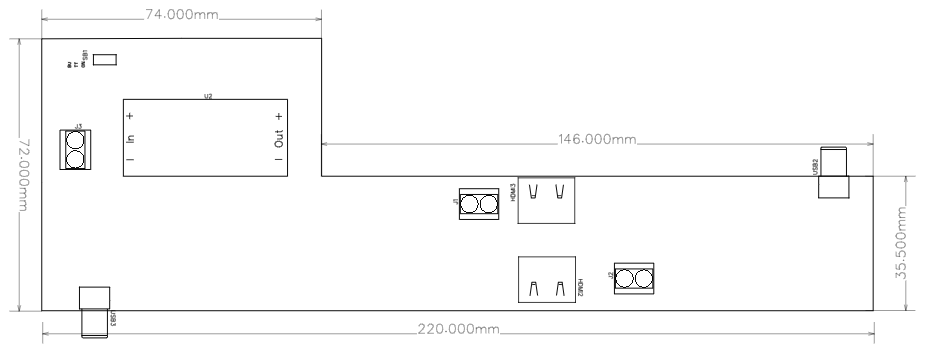
\includegraphics[scale=0.5]{figuras/PCB_Maleta.png}
  \caption{ Dimensões da PCI do circuito da central de controle.} 
  {\footnotesize Fonte : Autor } 
  \label{fig:PCIMaleta}
\end{figure}

\begin{figure}[H]
  \centering
  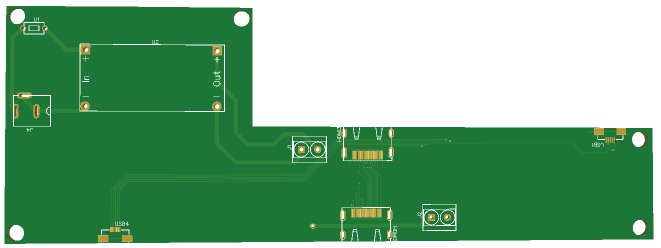
\includegraphics[scale=0.4]{figuras/PDFs/final eletronica/maleta_top.png}
    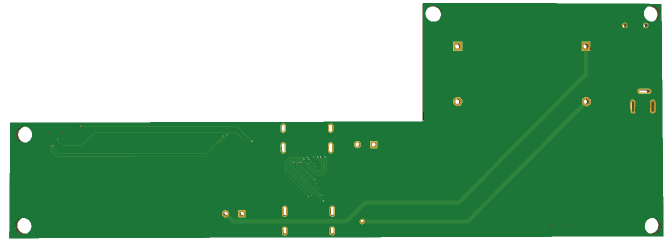
\includegraphics[scale=0.4]{figuras/PDFs/final eletronica/maleta_bottom.png}
  \caption{PCI do circuito interno do foguete. } 
  {\footnotesize Fonte : Autor } 
  \label{fig:PCB_controle}
\end{figure}
